%==============================================================
% Fundamentos Matemáticos del Aprendizaje Automático
% Tesina de Licenciatura — Nicolas Silva Nash
% Universidad Nacional del Comahue
%
% Uso: pdflatex presentacion.tex
% Requiere: pgfplots, tikz, babel(spanish), lmodern
%==============================================================
\documentclass[aspectratio=169, 10pt]{beamer}
%\documentclass[aspectratio=169,10pt,handout]{beamer}
%--------------------------------------------------------------
% TEMA Y PALETA DE COLORES (azul UNCo)
%--------------------------------------------------------------
\usetheme{Madrid}
\usepackage{xcolor}
\usepackage{amsmath}
\DeclareMathOperator{\sgn}{sgn}
\definecolor{uncoBlue}{RGB}{0,82,156}
\definecolor{uncoDark}{RGB}{0,50,100}
\colorlet{accentblue}{uncoBlue}
\colorlet{primaryblue}{uncoBlue}

\setbeamercolor{palette primary}  {bg=uncoBlue, fg=white}
\setbeamercolor{palette secondary}{bg=uncoDark, fg=white}
\setbeamercolor{palette tertiary} {bg=uncoBlue!80, fg=white}
\setbeamercolor{structure}        {fg=uncoBlue}
\setbeamercolor{block title}      {bg=uncoBlue, fg=white}
\setbeamercolor{block body}       {bg=uncoBlue!8}
\setbeamercolor{lightbg}          {bg=uncoBlue!8, fg=black}
\setbeamercolor{alerted text}     {fg=red!75!black}

%--------------------------------------------------------------
% PAQUETES
%--------------------------------------------------------------
\usepackage[spanish,es-noquoting]{babel}
\usepackage[utf8]{inputenc}
\usepackage{amsmath, amssymb}
\usepackage{mathtools}
\usepackage{lmodern}
\usepackage{graphicx}
\graphicspath{{images/}}
\usepackage{subfig}
\usepackage{animate}
\usepackage{tikz}
\usepackage{pgfplots}
\pgfplotsset{compat=1.18}
\usetikzlibrary{arrows.meta, positioning, shapes.geometric, shadows}

%--------------------------------------------------------------
% METADATOS
%--------------------------------------------------------------
\title[Fundamentos Matemáticos del Aprendizaje Automático]{%
  \Large\textbf{Fundamentos Matemáticos\\[0.4em]del Aprendizaje Automático}}

\large\author[Nicolas Silva Nash]{Nicolas Silva Nash}

\institute[UNCo -- Departamento de Matemática]{%
  Departamento de Matemática\\
  Universidad Nacional del Comahue\\[0.5em]
  {\footnotesize
    \textbf{Director:}~Dr.~Luis Nowak\qquad
    \textbf{Codirectora:}~Dra.~Alejandra Perini}}

\date{Defensa de Tesina de Licenciatura}

\newcommand{\rotuloslide}[3]{%
  \begin{frame}[plain]
    \begin{tikzpicture}[remember picture, overlay]
      \fill[uncoBlue!7] (current page.south west) rectangle (current page.north east);
      \fill[uncoBlue] (current page.north west) rectangle ([yshift=-1.05cm]current page.north east);
      \fill[uncoDark] (current page.south west) rectangle ([yshift=0.45cm]current page.south east);

      \node[
        anchor=north west,
        text=white,
        font=\Large\bfseries
      ] at ([xshift=0.85cm,yshift=-0.28cm]current page.north west) {#1};

      \node[
        anchor=center,
        text=uncoBlue,
        align=center,
        text width=0.82\paperwidth,
        font=\huge\bfseries
      ] at ([yshift=0.25cm]current page.center) {#2};

      \node[
        anchor=north,
        text=uncoDark,
        align=center,
        text width=0.72\paperwidth,
        font=\large
      ] at ([yshift=-0.85cm]current page.center) {#3};
    \end{tikzpicture}
  \end{frame}
}

\titlegraphic{%
  
\includegraphics[height=1.25cm,keepaspectratio]{\detokenize{../1. LaTeX/Images/logo_matematica_faea.png}}\hspace{1.5cm}%
  
\includegraphics[height=1.25cm,keepaspectratio]{\detokenize{../1. LaTeX/Images/logo_unco.png}}}

%==============================================================
\begin{document}
%==============================================================

% ─────────────────────────────────────────────────────────────
% BLOQUE 1: EL MAPA Y EL TERRITORIO
% ─────────────────────────────────────────────────────────────

%--------------------------------------------------------------
% DIAPOSITIVA 1 — TÍTULO
%--------------------------------------------------------------
\begin{frame}
  \titlepage
\end{frame}

\begin{frame}{Temario}
  \begin{enumerate}
    \setlength{\itemsep}{0.75em}
    \item \textbf{Aprendizaje automático:} qué significa aprender a partir de ejemplos.
    %\item \textbf{Clasificación binaria:} datos, etiquetas, clasificadores, riesgo y clasificador de Bayes.
    \item \textbf{Conceptos del aprendizaje:} generalización, riesgo empírico, consistencia y dilemas.
    \item \textbf{Teoría VC:} ley uniforme, fragmentación y dimensión VC.
    \item \textbf{Límites y panorama actual:} no hay almuerzos gratis y la paradoja moderna.
  \end{enumerate}
\end{frame}


\rotuloslide{01}{Aprendizaje automático}{Qué significa aprender a partir de ejemplos}

\begin{frame}
\centering
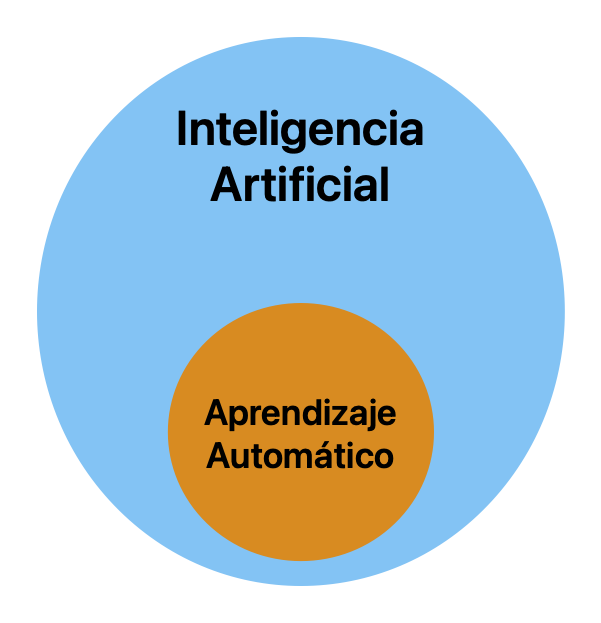
\includegraphics[height=0.8\textheight,keepaspectratio]{images/ml ai diagram.png}
\end{frame}

\begin{frame}
\centering
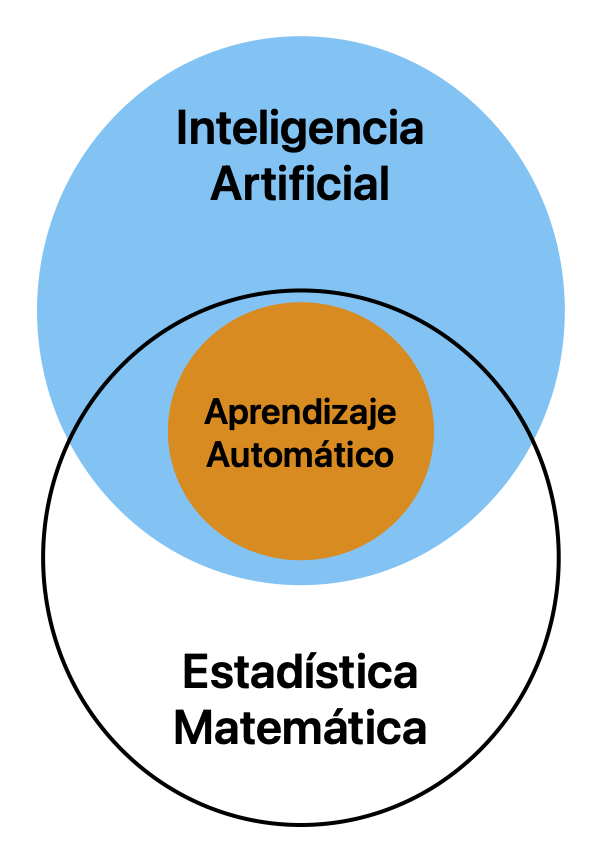
\includegraphics[height=0.8\textheight,keepaspectratio]{images/ml ai math diagram.png}
\end{frame}

\begin{frame}
  \begin{columns}[c]
    \begin{column}{0.5\textwidth}
      \centering
      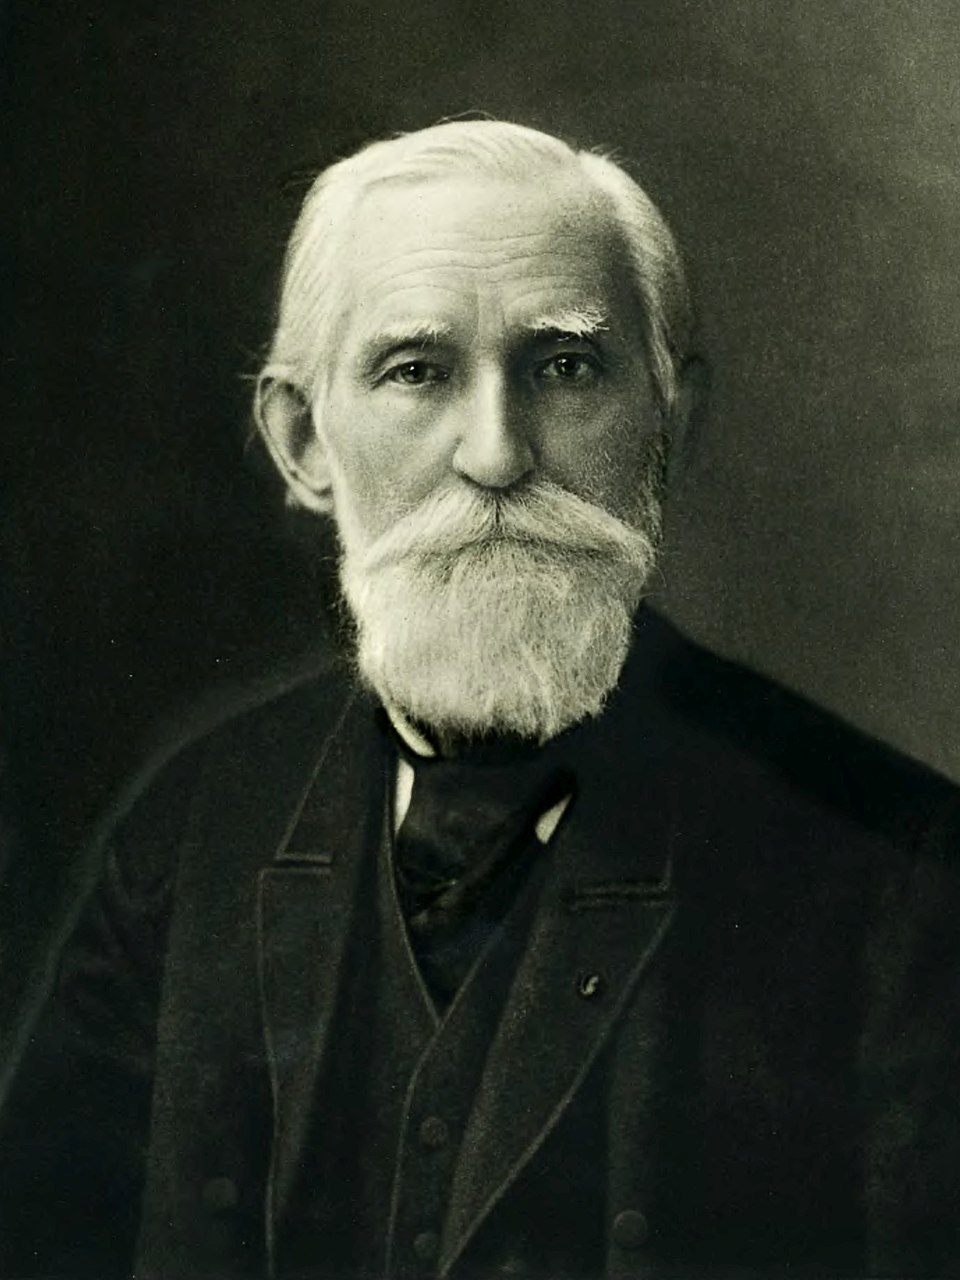
\includegraphics[width=0.75\linewidth,keepaspectratio]{images/chebyshev.jpg}

      \vspace{0.4em}
      \small Pafnuty Chebyshev
    \end{column}
    \begin{column}{0.5\textwidth}
      \centering
      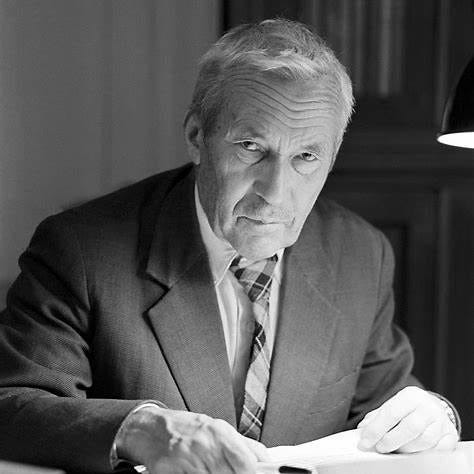
\includegraphics[width=0.82\linewidth,keepaspectratio]{images/kolmogorov.jpg}

      \vspace{0.4em}
      \small Andrey Kolmogorov
    \end{column}
  \end{columns}
\end{frame}

\begin{frame}[plain]
  \begin{columns}[c]
  \begin{column}{0.45\textwidth}
    \centering
    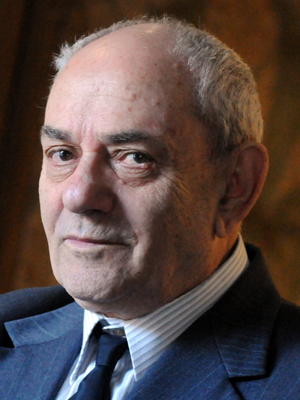
\includegraphics[height=0.8\paperheight,keepaspectratio]{images/Vapnik.png}\\[-0.2em]
    {\scriptsize Vladimir Vapnik}
  \end{column}
  \begin{column}{0.45\textwidth}
    \centering
    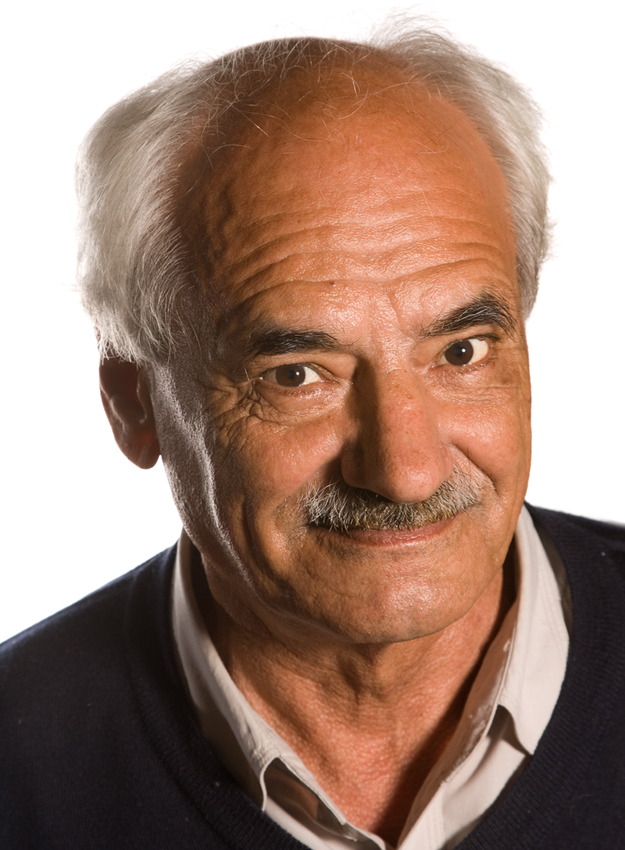
\includegraphics[height=0.8\paperheight,keepaspectratio]{images/Chervonenkis.JPG}\\[-0.2em]
    {\scriptsize Alexey Chervonenkis}
  \end{column}
\end{columns}
\end{frame}


\begin{frame}{¿Qué Entendemos por Aprendizaje?}
\large
        El aprendizaje es el proceso a través del cual pueden inferirse reglas generales a partir de ejemplos.\\

\bigskip
\pause       
  Nos interesa entender como una una computadora puede resolver ciertos problemas:
  \begin{itemize}
    \pause 
    \item sin conocer las reglas explícitamente de antemano,
    \pause 
    \item a partir de ejemplos,
    \pause 
    \item a través de un algoritmo de aprendizaje.
  \end{itemize} 

\end{frame}

% \begin{frame}[plain]
%   \IfFileExists{images/frames/frame_180.png}{%
%     \includegraphics[width=\paperwidth,height=\paperheight]{images/frames/frame_180.png}%
%     \begin{tikzpicture}[remember picture,overlay]
%       \node[
%         anchor=south,
%         fill=black,
%         fill opacity=0.58,
%         text opacity=1,
%         rounded corners=2pt,
%         inner sep=7pt,
%         text=white,
%         text width=0.9\paperwidth,
%         align=center
%       ] at ([yshift=0.7cm]current page.south) {\footnotesize
%         \textbf{Proceso Gaussiano en tiempo real:} cada nuevo dato observado actualiza la media y la incertidumbre del modelo, refinando de forma progresiva su predicci\'on.
%       };
%     \end{tikzpicture}
%   }{}
% \end{frame}

%--------------------------------------------------------------
% DIAPOSITIVA 3 — LAS MÁQUINAS APRENDEN
%--------------------------------------------------------------
\begin{frame}{¿Qué significa que una máquina aprenda a clasificar objetos?}
  \begin{columns}[T]

    \begin{column}{0.52\textwidth}
      \centering
      \IfFileExists{images/face_recognition.png}{%
        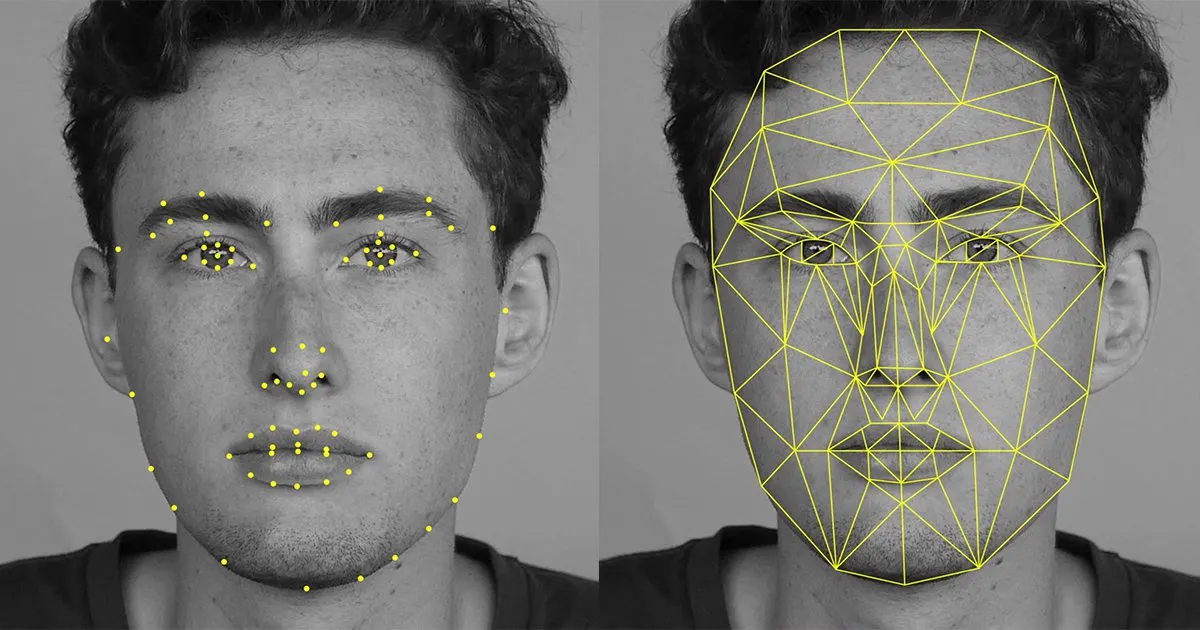
\includegraphics[width=\linewidth]{images/face_recognition.png}%
      }{%
        \begin{block}{Imagen no disponible}
          \centering
          \small No se encontró \texttt{images/face\_recognition.png}.
        \end{block}
      }
      {\scriptsize\textcolor{gray}{Reconocimiento facial mediante landmarks geométricos.}}
    \end{column}

    \begin{column}{0.46\textwidth}
      \vspace{0.4em}
      \begin{itemize}
        \setlength{\itemsep}{0.8em}
        \item A partir de \textbf{ejemplos}, la máquina construye una regla
          de decisión.
          \pause
        \item No se programa explícitamente la respuesta: se \textbf{infiere} desde los datos.
        \pause
        \item El desafío matemático: garantizar que la regla
          \textbf{generalice} a casos nuevos.
      \end{itemize}

      \vspace{0.8em}
      \centering
      \pause
      \large\alert{¿Cuándo y por qué funciona?}
    \end{column}

  \end{columns}
\end{frame}

%--------------------------------------------------------------
% DIAPOSITIVA 3b — ANIMACIÓN: LA MÁQUINA APRENDE
%--------------------------------------------------------------

% \begin{frame}{La Máquina Aprende: Ajuste Progresivo}
%   \centering
%   % Fallback para compilar aun cuando no exista la secuencia de cuadros.
%   \IfFileExists{images/frames/frame_000.png}{%
%     \animategraphics[loop, autoplay, width=0.82\linewidth]{12}{images/frames/frame_}{000}{180}%
%   }{%
%     \begin{block}{Animación no disponible}
%       \centering
%       \small No se encontraron archivos en \texttt{images/frames/frame\_***}.
%     \end{block}
%   }

%   \vspace{0.3em}
%   {\scriptsize\textcolor{gray}{Proceso Gaussiano ajustándose progresivamente a los datos de entrenamiento.}}
% \end{frame}

\begin{frame}{Clasificación: Planteo del Problema}
  \vspace{0.4em}
  \begin{center}
    \begin{minipage}{0.92\textwidth}

        Consideremos dos espacios de variables: $X$, llamado espacio de entrada, e $Y$, el espacio de etiquetas.\\

        \bigskip
        \pause
        En un problema de
        clasificación, deseamos poder etiquetar correctamente elementos de $X$ con los valores de $Y$.\\


    \end{minipage}
  \end{center}
\end{frame}

\begin{frame}

\centering
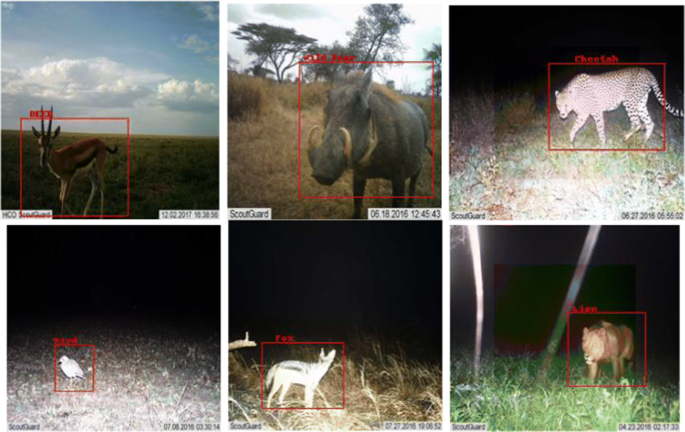
\includegraphics[height=0.8\textheight,keepaspectratio]{images/animal_classification.png}

{\scriptsize\textcolor{gray}{Reconocimiento de distintos tipos de animales}}


\end{frame}


%\rotuloslide{02}{Clasificación binaria}{Datos, etiquetas, riesgo y clasificador de Bayes}

\begin{frame}{Clasificación: Datos y Clasificador}
  \vspace{0.4em}
  \begin{center}
    \begin{minipage}{0.92\textwidth}
        Asumimos que entre el espacio de entrada y el espacio de etiquetas hay una distribución
        de probabilidad conjunta $P=P(X,Y)$.\\

        \pause
        Con el fin de aprender, a un algoritmo se le muestran ejemplos de imágenes y sus respectivas
        etiquetas $(X_1,Y_1), (X_2,Y_2), \ldots, (X_n,Y_n)$, a partir de los cuales este debe
        encontrar una función $f : X \to Y$, que comete la menor cantidad de errores posibles. \\

        \pause
        A esta función $f$ la llamamos clasificador.\\

        \pause
        A fin de simplificar la teoría, nos centraremos en el más sencillo de los problemas del Machine Learning, el de
        \textbf{clasificación binaria}.\pause En este caso, tendremos dos categorías de etiquetas, por lo que
        $$
          Y = \{-1,+1\}
        $$

    \end{minipage}
  \end{center}
\end{frame}

\begin{frame}

      \centering
  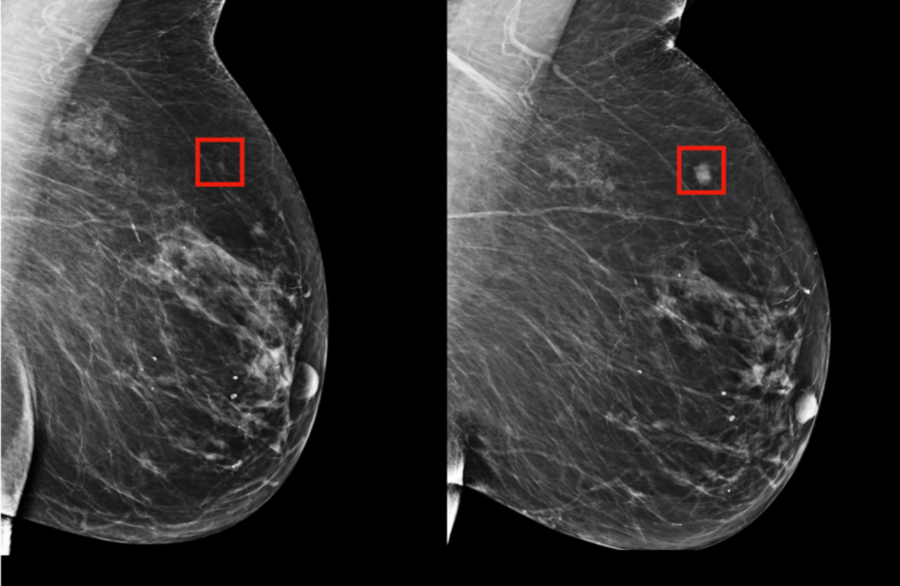
\includegraphics[height=0.8\textheight,keepaspectratio]{images/BreastCancerAI.png}

  {\scriptsize\textcolor{gray}{Clasificación de imágenes médicas para diagnóstico de cáncer de mama.}}
\end{frame}
\begin{frame}

      \centering
      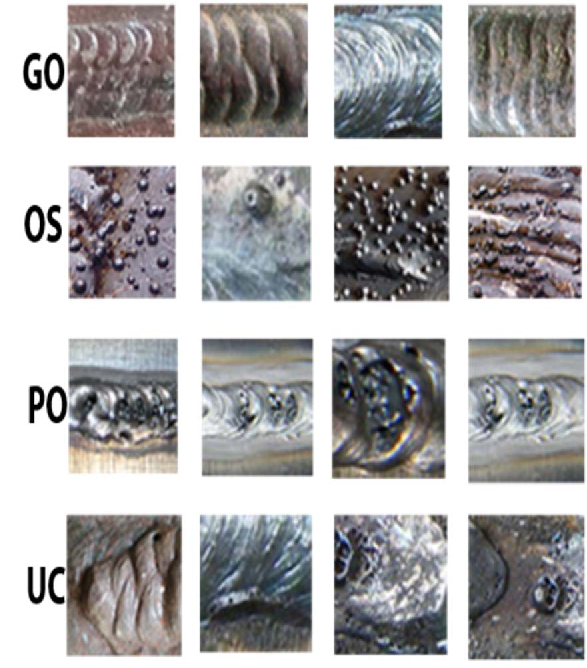
\includegraphics[width=\linewidth,height=0.84\textheight,keepaspectratio]{images/weldingDefects.png}

      \vspace{0.2em}
      {\scriptsize\textcolor{gray}{Clasificación de defectos en soldaduras.}}
\end{frame}

\begin{frame}{Clasificación: Suposiciones básicas}
  \begin{itemize}
    \large
    \setlength{\itemsep}{0.45em}
    \item \textbf{No aplicamos restricciones sobre $P$:} no suponemos una forma paramétrica para la distribución que genera los datos.
    \pause
    \item \textbf{Etiquetas no determinísticas:} modelamos $Y$ mediante probabilidades condicionales $P(Y=1\mid X=x)$.
      % \begin{itemize}
      %   \item Puede existir solapamiento entre las clases. (ej: imágenes lejanas de perros y gatos con características similares).
      %   \item En la práctica, hay ruido en las etiquetas. (ej: distintos etiquetadores humanos no coincidiendo en si un email es spam;
      %    errores de etiquetado).
      % \end{itemize}
    \pause
    \item \textbf{Muestreo iid:} los ejemplos se toman de manera independiente e idénticamente distribuida.
    \pause
    \item \textbf{Distribución fija:} asumimos que el mecanismo que genera los datos no cambia entre entrenamiento y uso.
  %   \pause
  %   \item \textbf{$P$ desconocida:} solo accedemos a la distribución a través de una muestra finita de datos. El valor de la teoría
  %   estará en entender bajo qué condiciones podremos inferir algo sobre $P$.
  \end{itemize}
\end{frame}



%--------------------------------------------------------------%--------------------------------------------------------------
%--------------------------------------------------------------%--------------------------------------------------------------
%--------------------------------------------------------------%--------------------------------------------------------------


%--------------------------------------------------------------
% DIAPOSITIVA 4 — FORMALIZANDO EL TERRENO DE JUEGO
%--------------------------------------------------------------
\begin{frame}{Formalizando el Terreno de Juego}

      \begin{block}{Objetivo}
        \Large
        Construir $f:X\to Y$ que generalice
        a puntos \textbf{no vistos}.
      \end{block}

      \vspace{0.9em}
      \pause

      \begin{alertblock}{Diferencia clave con Estadística clásica}
        \Large
        Somos \textbf{agnósticos} respecto a $P$:
        no asumimos ninguna forma paramétrica.
        Conocemos a la distribución $P$ \textit{solo} a través de la muestra finita.
      \end{alertblock}

\end{frame}


\rotuloslide{02}{Conceptos del aprendizaje}{Generalización, consistencia y dilemas del aprendizaje}

\begin{frame}
  \centering
  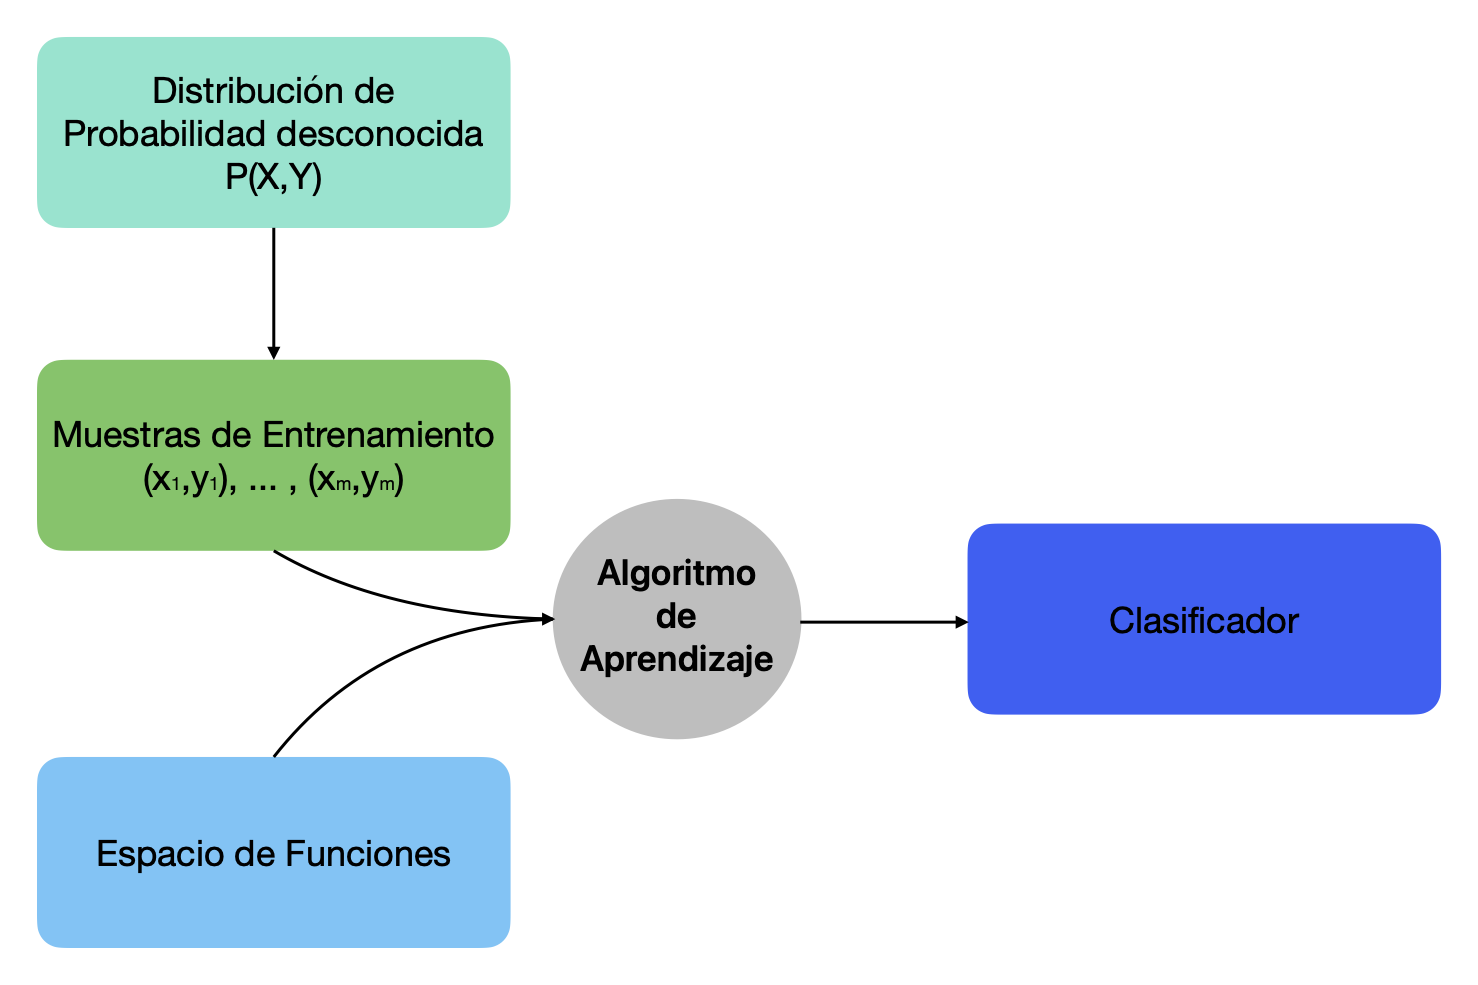
\includegraphics[height=0.86\textheight,keepaspectratio]{images/diagram aprendizaje.png}
\end{frame}


%--------------------------------------------------------------
% DIAPOSITIVA 4 — ¿QUÉ SIGNIFICA EQUIVOCARSE?
%--------------------------------------------------------------
\begin{frame}{¿Qué Significa Equivocarse?: Función de Pérdida}

  Para medir la efectividad de la función clasificadora, definimos una Función de Pérdida $\ell$.\\
\pause
  En el caso binario, la función más sencilla es
\begin{block}{Función de pérdida 0-1}
  \Large
  \[
          \ell\bigl(X,Y,f(X)\bigr) \;:=\;
        \begin{cases}
          1 & \text{si } f(X) \neq Y \\
          0 & \text{si } f(X) = Y
        \end{cases}
      \]
\end{block}
\pause
Por convención, una pérdida igual a 0 implica una clasificación perfecta y valores
mayores implican peor clasificación. \\

\end{frame}
\begin{frame}{¿Qué Significa Equivocarse?: Función de Riesgo}
Mientras que la función de pérdida mide el error del clasificador en un punto
individual $x \in X$, llamamos riesgo, $R$, del clasificador a la pérdida esperada
sobre todos los datos generados por la distribución de probabilidad P
\pause
      \begin{block}{Riesgo}
        \Large
      \[
        \mathcal{R}(f)
        \;:=\;
        \mathbb{E}_P\bigl[\,\ell(X,Y,f(X))\,\bigr] = \int \ell(X,Y,f(X))\,dP(X,Y)
      \]

      \end{block}
\pause
\bigskip
El mejor clasificador posible minimiza $\mathcal{R}$.\\

\pause
\bigskip
\begin{alertblock}{ }
  Es decir, el aprendizaje implica un desafío de optimización en dónde deseamos hallar el mínimo de la función de
riesgo.
\end{alertblock}

\end{frame}


% %  \end{column}

%     %% — Columna derecha: el obstáculo y la solución provisional
%     \begin{column}{0.45\textwidth}
%       \begin{alertblock}{El obstáculo central}
%         Calcular $\mathcal{R}(f)$ requiere conocer\\
%         $P(X,Y)$\ldots\\[0.4em]
%         \centering\large\textbf{que no conocemos.}
%       \end{alertblock}

%       \vspace{0.6em}

%       \begin{block}{Lo que sí podemos hacer}
%         Aproximar $\mathcal{R}(f)$ con la \textbf{pérdida promedio}
%         sobre los datos de entrenamiento:
%         \[
%           \mathcal{R}(f)
%           \;\approx\;
%           \mathcal{R}_{\mathrm{emp}}(f)
%         \]
%       \end{block}
%     \end{column}


%--------------------------------------------------------------
% DIAPOSITIVA 5 — EL IDEAL INALCANZABLE (Clasificador de Bayes)
%--------------------------------------------------------------
\begin{frame}{El Ideal Inalcanzable: $f_{\mathrm{Bayes}}$}

      \begin{block}{Clasificador de Bayes:}
        \large
      \[
        f_{\mathrm{Bayes}}(x) \;:=\;
        \begin{cases}
          +1 & \text{si } P(Y=1\mid X=x)\;\geq\;\tfrac{1}{2}\\[4pt]
          -1 & \text{en otro caso}
        \end{cases}
      \]
      \end{block}
\pause
      \vspace{0.5em}
      \begin{itemize}
        \setlength{\itemsep}{0.5em}
        \item Minimiza $\mathcal{R}(f)$ sobre \textbf{todas} las funciones medibles.
        \pause
        \item Asigna siempre la etiqueta más probable dado $x$.
        \pause
        \item Es el \textbf{techo teórico} de cualquier clasificador.
      \end{itemize}
    \pause
      \begin{alertblock}{¿Por qué es inalcanzable?}
        \large
        Requiere conocer $P(X, Y)$,\textbf{ que es exactamente lo que desconocemos}.
      \end{alertblock}
\end{frame}

\begin{frame}
  \begin{block}{Función Medible (Clasificador)}
    Sea $(\mathcal{X}, \Sigma)$ un espacio medible, donde $\mathcal{X}$ es el espacio de características de entrada y $\Sigma$ es su $\sigma$-álgebra asociada (típicamente la $\sigma$-álgebra de Borel). Una regla de clasificación $f: \mathcal{X} \to \{0, 1\}$ es una \textbf{función medible} si la preimagen de cada conjunto medible en el espacio de etiquetas pertenece a $\Sigma$.
    \end{block}
    \begin{block}{}
Dado que el espacio de etiquetas es discreto y finito, esto se simplifica significativamente: $f$ es medible si y solo si las regiones de decisión que define en el espacio de entrada son conjuntos medibles:
\[
\{x \in \mathcal{X} : f(x) = 1\} \in \Sigma \quad \text{y} \quad \{x \in \mathcal{X} : f(x) = 0\} \in \Sigma
\]
  \end{block}


\end{frame}

\begin{frame}{Definición del problema de clasificación binaria}
  Si el clasificador de Bayes es incomputable en la práctica, ¿Qué utilidad tiene definirlo?\\
\pause
\bigskip
  Lo hacemos porque nos permite definir el problema que estamos tratando.

\pause
\bigskip
  \begin{block}{Definición}
  \Large
  Dado un conjunto de datos de entrenamiento $ \{ (X_1,Y_1), \dots ,(X_n, Y_m)\}$
obtenidos iid de una distribución $P$, y dada una función de pérdida $\ell$, deseamos construir una función clasificadora
$f:X\rightarrow Y$ cuyo riesgo $\mathcal{R}(f)$ sea lo más cercano posible al riesgo de $f_{\text{Bayes}}$.\\

Llamamos a este problema \textbf{clasificación binaria}.
  \end{block}
\pause
\bigskip
Pero... ¿Cómo construímos esta función clasificadora?
\end{frame}

\begin{frame}{Algoritmo de Aprendizaje}
  \begin{block}{Definición}
    \Large
    Llamamos \textbf{algoritmo de aprendizaje} a todo procedimiento matemático que, dado un conjunto
de datos de entrenamiento $(X_i,Y_i)$, devuelve una función clasificadora $f$ sobre el espacio de entrada $X$ 
y el espacio de etiquetas $Y$ del que
provienen los datos.
  \end{block}
\pause
\bigskip
  El algoritmo define la forma de la función clasificadora. En general, a través de este determinamos al espacio funcional $\mathcal{F}$ de
  donde extraemos los distintos clasificadores del proceso de aprendizaje.
\end{frame}


  \begin{frame}{Algoritmo de Aprendizaje}
  \begin{block}{Ejemplo: El perceptrón de Rosenblatt}
Dado un conjunto de entrenamiento $S = \{(\mathbf{x}_i, y_i)\}_{i=1}^n \subset \mathbb{R}^d \times \{0, 1\}$,
el Perceptrón se define como un clasificador binario $h: \mathbb{R}^d \to \{-1, 1\}$ mediante la siguiente función:

\begin{equation*}
    h_{\mathbf{w}}(\mathbf{x}) = \sgn(\mathbf{w}^T \mathbf{x} > 0)
\end{equation*}

Donde $\mathbf{w} \in \mathbb{R}^d$ es el vector de pesos
y $\sgn(\cdot)$ denota la función Signum. El aprendizaje de los parámetros se realiza a través
de una regla de actualización iterativa. Para cada muestra $(\mathbf{x}_i, y_i)$, la actualización se define como:

\begin{align*}
    \mathbf{w}^{(t+1)} &\gets \mathbf{w}^{(t)} + \eta (y_i - \hat{y}_i) \mathbf{x}_i
\end{align*}

donde $\hat{y}_i = h_{\mathbf{w}^{(t)}}(\mathbf{x}_i)$ es la predicción actual y $\eta \in (0, 1]$
es llamada la tasa de aprendizaje.

  \end{block}
\end{frame}

\begin{frame}
  \begin{figure}
    \centering
    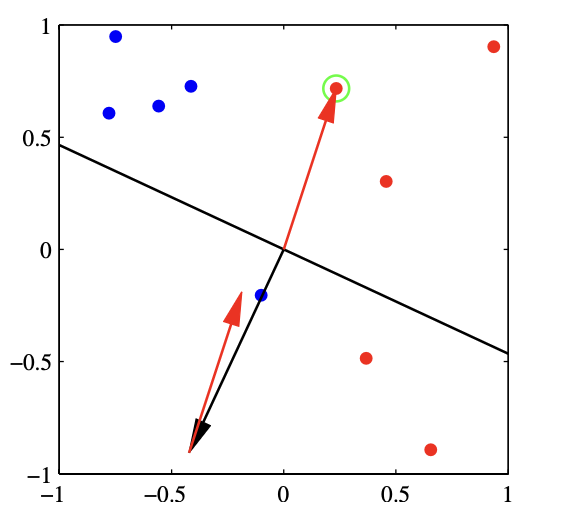
\includegraphics[width=0.27\textwidth]{images/perceptron 1.png}\hspace{0.025\textwidth}
    \pause
    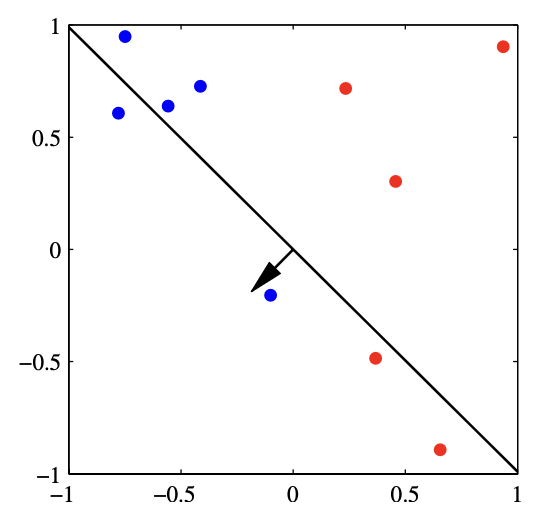
\includegraphics[width=0.27\textwidth]{images/perceptron 2.png}\\[0.2em]
    \pause
    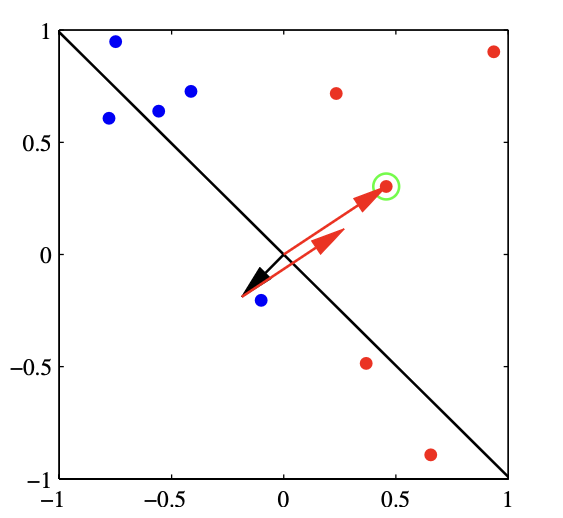
\includegraphics[width=0.27\textwidth]{images/perceptron 3.png}\hspace{0.025\textwidth}
    \pause
    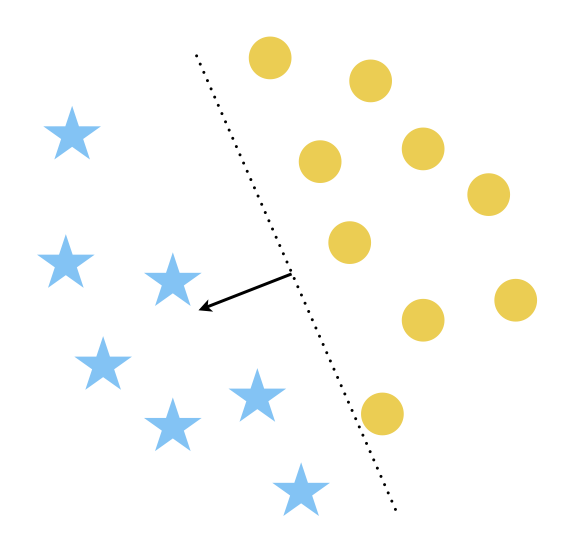
\includegraphics[width=0.27\textwidth]{images/perceptron 4.png}
  \end{figure}
\end{frame}

% \begin{frame}

% \begin{tikzpicture}[
%     font=\sffamily\small,
%     >=Stealth,
%     node distance=1.2cm and 1.8cm,
%     % Modern styling for boxes
%     box/.style={
%         rectangle, draw=blue!50!black!70, fill=blue!5, very thick,
%         inner sep=8pt, text centered, align=center, rounded corners=4pt,
%         minimum width=3.5cm, drop shadow={opacity=0.15}
%     },
%     % Styling for the central Learning Algorithm
%     circlebox/.style={
%         circle, draw=orange!80!black, fill=orange!10, very thick,
%         inner sep=5pt, text centered, align=center, minimum size=2.8cm,
%         drop shadow={opacity=0.15}
%     },
%     % Subtle styling for the Error Measure
%     errorbox/.style={
%         rectangle, draw=gray!60, fill=gray!5, thick,
%         inner sep=5pt, rounded corners=10pt
%     }
% ]

%     % --- NODES ---
%     \node [box] (target) {
%         \textbf{Target Distribution}\\
%         $P(y \mid \mathbf{x})$
%     };

%     \node [box, right=of target] (input) {
%         \textbf{Input Distribution}\\
%         $P(\mathbf{x})$
%     };

%     \node [box, below=of target] (examples) {
%         \textbf{Training Examples}\\
%         $\mathcal{D} = \{(\mathbf{x}_1, y_1), \dots, (\mathbf{x}_N, y_N)\}$
%     };

%     \node [circlebox, below right=1cm and -0.2cm of examples] (algo) {
%         \textbf{Learning}\\
%         \textbf{Algorithm}\\
%         $\mathcal{A}$
%     };

%     \node [box, below=2cm of examples] (hyp_set) {
%         \textbf{Hypothesis Set}\\
%         $\mathcal{H}$
%     };

%     \node [box, right=2.2cm of algo] (final) {
%         \textbf{Final Hypothesis}\\
%         $g \approx f$
%     };

%     \node [errorbox, above=0.8cm of algo] (error) {Error Measure};

%     % --- ARROWS ---
%     \draw [->, thick] (target) -- (examples);
%     \draw [->, thick] (input.west) -- node[above, font=\scriptsize] {$\mathbf{x}_1, \dots, \mathbf{x}_N$} (examples.east);

%     % Path from Input Dist to Final Hypothesis
%     \draw [->, thick] (input.south) -- ++(0,-3.4) node[right, pos=0.85] {$\mathbf{x}$} -- (final.north);

%     % Converging to Algorithm
%     \draw [->, thick] (examples.south) to [out=-90, in=150] (algo.150);
%     \draw [->, thick] (hyp_set.north) to [out=90, in=210] (algo.210);

%     \draw [->, thick] (algo) -- (final);
%     \draw [->, thick] (error) -- (algo);

%     % Arc from Error to Final
%     \draw [->, thick, dashed, color=gray] (error.east) to [out=0, in=120] (final.north west);

% \end{tikzpicture}
% \end{frame}


%\rotuloslide{03}{Conceptos del aprendizaje}{Generalización, riesgo empírico, consistencia y dilemas}

\begin{frame}{Consistencia}

    % Sea $(X_i,Y_i)_{i\in\mathbb{N}}$ una sucesión infinita de puntos de entrenamiento que han sido tomados iid de una distribución $P$.
    % Sea $\ell$ una función de pérdida. Por cada $n\in \mathbb{N}$, sea $f_n$ un clasificador construido por algún algoritmo de aprendizaje
    % usando los primeros $n$ puntos de entrenamiento. Sea $\mathcal{F}$ el espacio funcional de todos los posibles clasificadores según
    % el mecanismo de construcción del algoritmo. \pause Entonces
    % \bigskip
    \begin{enumerate}
      {\large
    \item  Sea $\mathcal{R}(f_{\mathcal{F}})$ clasificador que minimiza el riesgo en $\mathcal{F}$. El algoritmo de aprendizaje se dice 
    \textbf{consistente con respecto a $\mathcal{F}$ y a $P$} si para todo $\varepsilon>0$:
     \[
     P\left(\mathcal{R}(f_n)-\mathcal{R}(f_{\mathcal{F}})>\varepsilon\right) \rightarrow 0 \qquad \text{ cuando } \qquad n\rightarrow \infty
     \]
      }
     \pause

\[ \text{Es decir } P(\{\omega \in \Omega : |\mathcal{R}(f_n)(\omega) - \mathcal{R}(f_{\mathcal{F}})(\omega)| > \varepsilon\}) \rightarrow 0 \quad \text{ cuando } \quad n \rightarrow \infty \]
     \pause
     \bigskip
     {\large
     \item  El algoritmo de aprendizaje se dice \textbf{Bayes-consistente con respecto a $P$} si para todo $\varepsilon>0$
    \[
     P\left(\mathcal{R}(f_n)-\mathcal{R}(f_{\text{Bayes}})>\varepsilon\right) \rightarrow 0 \qquad \text{ cuando } \qquad n\rightarrow \infty
    \]
      }
      \pause
    \[ \text{Es decir } P(\{\omega \in \Omega : |\mathcal{R}(f_n)(\omega) - \mathcal{R}(f_{\text{Bayes}})(\omega)| > \varepsilon\}) \rightarrow 0 \quad \text{ cuando } \quad n \rightarrow \infty \]

    % \pause
    % \item  El algoritmo de aprendizaje se dice \textnormal{universalmente consistente con respecto a $\mathcal{F}$} si
    % es consistente con respecto a $\mathcal{F}$ para toda distribución de probabilidad $P$.
    % \pause
    % \item  El algoritmo de aprendizaje se dice \textnormal{universalmente Bayes-consistente } si
    % es Bayes-consistente para toda distribución de probabilidad $P$.
     \end{enumerate}

\end{frame}



\begin{frame}
  \Large
  \begin{alertblock}{Hay muchas cosas que no podemos calcular}
      No somos capaces de hallar al clasificador de Bayes.\\
      \pause
      En general, no podemos hallar explícitamente al mejor clasificador de un espacio funcional.\\
      \pause
      Ni siquiera podemos calcular el riesgo de un clasificador conocido.\\
      ...\\
      ¿Qué podemos hacer?
  \end{alertblock}
\pause
\bigskip
  Podemos “contar”  el número de errores del clasificador sobre los
datos de entrenamiento. \\

\end{frame}

\begin{frame}{Riesgo Empírico}
  \begin{block}{Definición}
    \large
    Sea $(X_i,Y_i)_{i=1}^n$ un conjunto de datos de entrenamiento, donde cada $(X_i,Y_i)$ es tomado iid de una distribución de probabilidad $P(X,Y)$. Sea
    $\ell$ una función de pérdida. Sea $f_n$ un clasificador binario construido a partir de ejemplos, luego
    de ser presentado con los primeros $n$ datos de entrenamiento.\\
\bigskip

    Entonces el \textbf{riesgo empírico} del clasificador $f$ es la pérdida promedio sobre los datos de entrenamiento, es decir
    \[
    R_{emp}(f) := \frac{1}{n} \sum_{i=1}^n \ell(X_i,Y_i,f(X_i))
    \]
\end{block}
\end{frame}


% \begin{frame}{Algoritmos de aprendizaje}
%   \begin{block}{Definición}
%     Llamamos \textbf{algoritmo de aprendizaje} a todo procedimiento matemático que, dado un conjunto
% de datos de entrenamiento $(X_i,Y_i)$, devuelve una función clasificadora $f$ sobre el espacio de entrada
% $\mathcal{X}$ y el espacio de etiquetas $\mathcal{Y}$ del que provienen los datos.
%   \end{block}

%   En la práctica, todo algoritmo de aprendizaje se construye sobre la función de pérdida previamente definida
%   para el problema dado. El objetivo del algoritmo es minimizar la pérdida promedio, es decir,
%   el riesgo empírico.

%   Usualmente llamamos \textbf{error de entrenamiento} al riesgo empírico por su relación con el algoritmo de aprendizaje.
%   \end{frame}


\begin{frame}
  \Large
  Desearíamos que el riesgo empírico se halle ``cerca'' del real, porque podríamos inferir la calidad de nuestro clasificador
  para toda la distribución y no solo en los datos de entrenamiento.\\
  \bigskip
  \pause
  Llamamos a esta idea \textbf{generalización}.\\
\pause
  \begin{block}{Generalización}
  
    Deseamos que
    \[
\mathcal{R}_{\text{emp}}(f) \approx \mathcal{R}(f)
    \]
  \end{block}

  \end{frame}


\begin{frame}{Generalización}
  \centering
  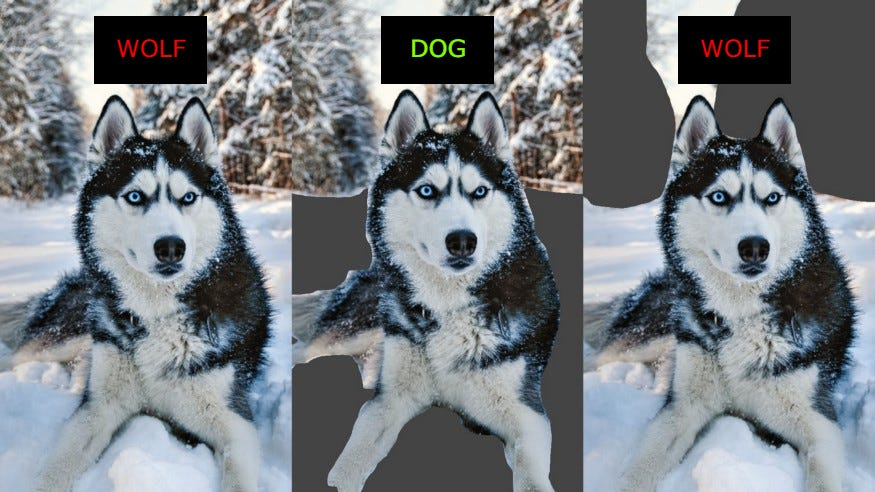
\includegraphics[width=0.92\textwidth,height=0.78\textheight,keepaspectratio]{images/wolf.jpg}
\end{frame}

\begin{frame}{El Dilema de la Complejidad}
  \begin{columns}

    %% — Columna izquierda: qué implica el tradeoff sesgo-varianza
    \begin{column}[c]{0.50\textwidth}

      \[
        \underbrace{\mathcal{R}(f_n) - \mathcal{R}(f_{\mathrm{Bayes}})}_{\text{lo que queremos reducir}}
      \]
      \[
        =\;
        \underbrace{\mathcal{R}(f_n) - \mathcal{R}(f_{\mathcal{F}})}_{\textcolor{uncoBlue}{\text{error de estimación}}}
        \;+\;
        \underbrace{\mathcal{R}(f_{\mathcal{F}}) - \mathcal{R}(f_{\mathrm{Bayes}})}_{\textcolor{red}{\text{error de aproximación}}}
      \]
    \end{column}
    \pause
    %% — Columna derecha: figura sesgo-varianza (Figura 2.3)
    \begin{column}{0.48\textwidth}
      \centering
      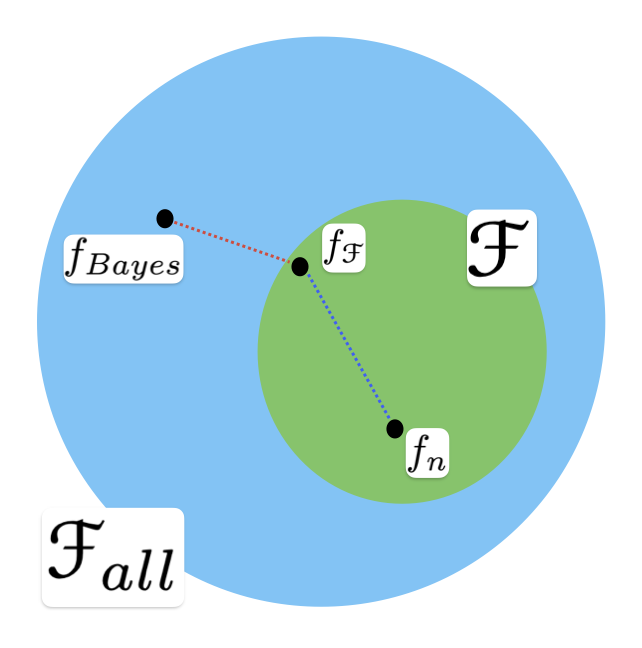
\includegraphics[width=\linewidth,keepaspectratio]{images/bias-variance tradeoff.png}

      {\scriptsize\textcolor{gray}{El error total puede ser descompuesto en dos componentes.}}
    \end{column}

  \end{columns}
\end{frame}

\begin{frame}{El Dilema Sesgo-Varianza}
  \begin{columns}[T]
    \begin{column}{0.50\textwidth}
      \begin{block}{ }
        \small
        \begin{itemize}
          \setlength{\itemsep}{0.35em}
          \item Si $\mathcal{F}$ es \textbf{poco compleja}, minimizamos el \textcolor{uncoBlue}{error de estimación} (alto sesgo).
          \item Si $\mathcal{F}$ es \textbf{muy compleja}, minimizamos el \textcolor{red}{error de aproximación} (alta varianza).
          \item La generalización mejora en un punto intermedio: \textbf{ni demasiado simple ni demasiado complejo}.
        \end{itemize}
      \end{block}
      \[
        \underbrace{\mathcal{R}(f_n) - \mathcal{R}(f_{\mathcal{F}})}_{\textcolor{uncoBlue}{\text{error de estimación}}}
        \;+\;
        \underbrace{\mathcal{R}(f_{\mathcal{F}}) - \mathcal{R}(f_{\mathrm{Bayes}})}_{\textcolor{red}{\text{error de aproximación}}}
      \]
    \end{column}
    \begin{column}{0.48\textwidth}
      \centering
      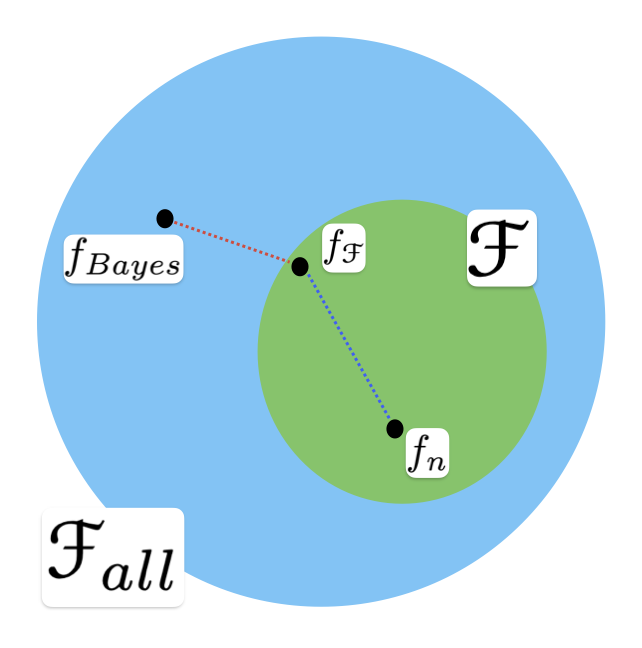
\includegraphics[width=\linewidth,keepaspectratio]{images/bias-variance tradeoff.png}

      {\scriptsize\textcolor{gray}{El error total puede ser descompuesto en dos componentes.}}
    \end{column}
  \end{columns}
\end{frame}

\begin{frame}{El Dilema Sesgo-Varianza}
  \begin{columns}[T]
    \begin{column}{0.50\textwidth}
      \begin{block}{ }
        \small
        \begin{itemize}
          \setlength{\itemsep}{0.35em}
          \item Si $\mathcal{F}$ es \textbf{poco compleja}, minimizamos el \textcolor{uncoBlue}{error de estimación} (alto sesgo).
          \item Si $\mathcal{F}$ es \textbf{muy compleja}, minimizamos el \textcolor{red}{error de aproximación} (alta varianza).
          \item La generalización mejora en un punto intermedio: \textbf{ni demasiado simple ni demasiado complejo}.
        \end{itemize}
      \end{block}
      \[
        \underbrace{\mathcal{R}(f_n) - \mathcal{R}(f_{\mathcal{F}})}_{\textcolor{uncoBlue}{\text{error de estimación}}}
        \;+\;
        \underbrace{\mathcal{R}(f_{\mathcal{F}}) - \mathcal{R}(f_{\mathrm{Bayes}})}_{\textcolor{red}{\text{error de aproximación}}}
      \]
    \end{column}

    %% — Columna derecha: figura sesgo-varianza (Figura 2.3)
    \begin{column}{0.48\textwidth}
      \centering
      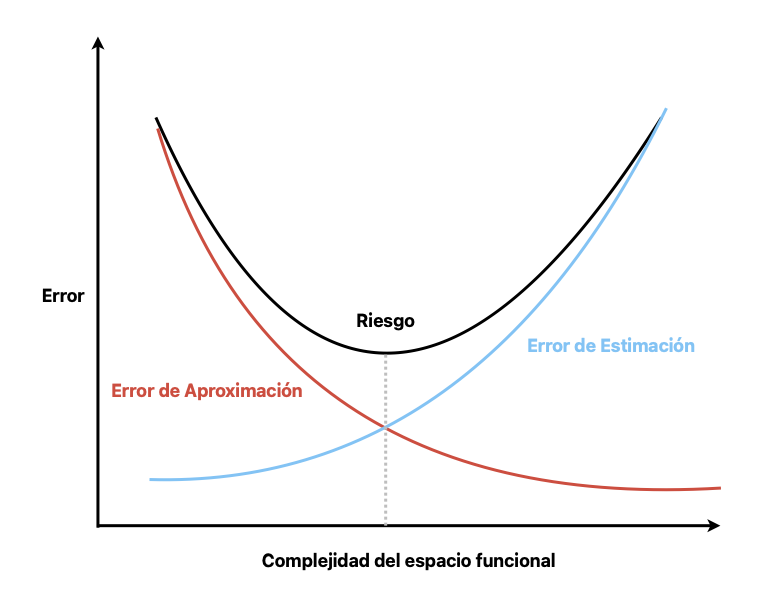
\includegraphics[width=\linewidth,keepaspectratio]{images/error de aproximación y de estimación.png}

      \vspace{0.1em}
      {\scriptsize\textcolor{gray}{El error de aproximación disminuye con la complejidad, 
      mientras que el error de estimación aumenta a partir de un punto \textit{óptimo}.}}
    \end{column}
  \end{columns}
\end{frame}

\begin{frame}{Subajuste y sobreajuste}
  \begin{figure}
    \centering
    \captionsetup[subfloat]{labelformat=empty,labelsep=none}
    \subfloat[\scriptsize Subajuste]{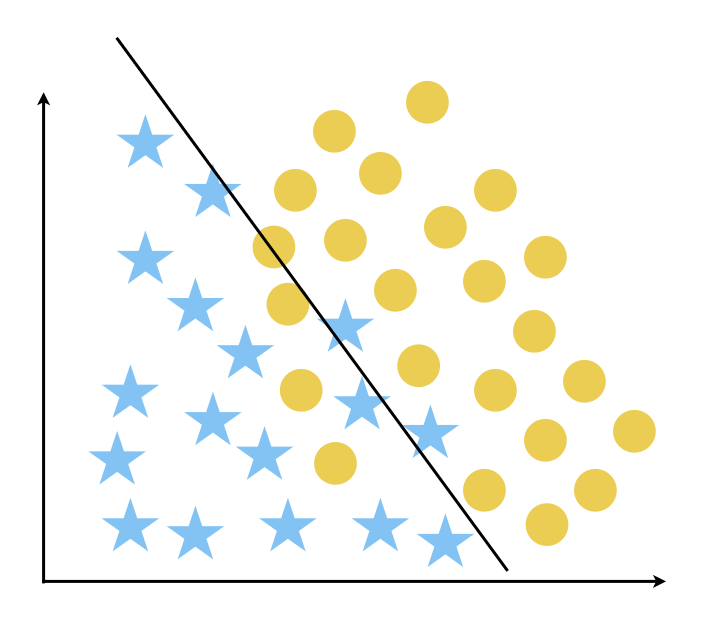
\includegraphics[width=0.31\textwidth]{images/classification underfitting.png}}\hspace{0.02\textwidth}
    \pause
    \subfloat[\scriptsize Sobreajuste]{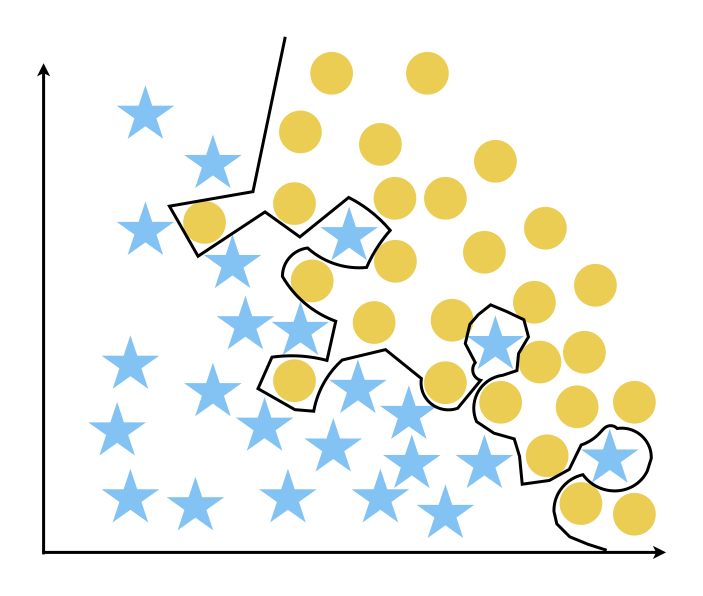
\includegraphics[width=0.31\textwidth]{images/classification overfitting.png}}
    \pause
    \subfloat[\scriptsize Balanceado]{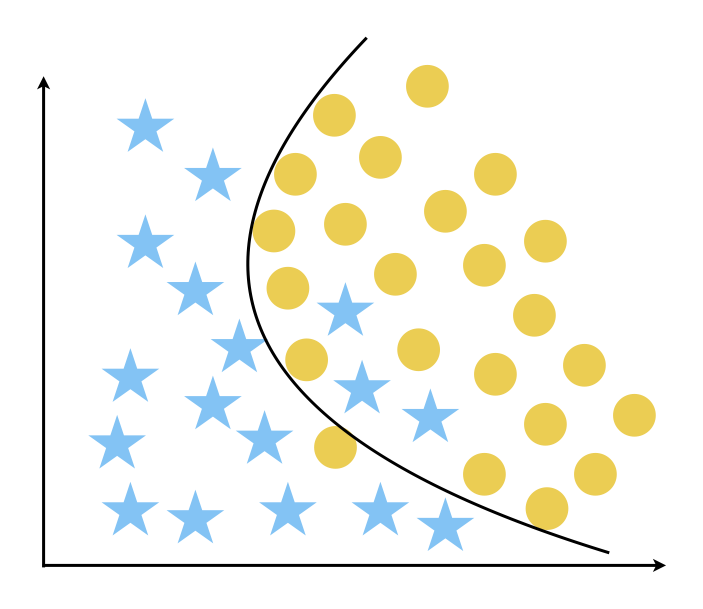
\includegraphics[width=0.31\textwidth]{images/classification balanced.png}}\hspace{0.02\textwidth}
  \end{figure}
\end{frame}


\begin{frame}{}
  \vfill
  \begin{center}
    \begin{minipage}{0.78\textwidth}
      \begin{block}{}
        {\large\itshape
        ``[Funes] había aprendido sin esfuerzo el inglés, el francés, el portugués, el latín.
        Sospecho, sin embargo, que no era muy capaz de pensar. Pensar es olvidar
        diferencias, es generalizar, abstraer. En el abarrotado mundo de Funes
        no había sino detalles, casi inmediatos.''
        }
        \vspace{0.5em}
        \begin{flushright}
      
          ---~Jorge Luis Borges,\\
          \textit{Funes el memorioso}
        \end{flushright}
      \end{block}
    \end{minipage}
  \end{center}
  \vfill
\end{frame}


\rotuloslide{04}{Teoría VC}{Ley uniforme, fragmentación y dimensión VC}

\begin{frame}{La Ley de los Grandes Números}
En su forma más simple, la ley de los grandes números
establece que, bajo condiciones suaves, la media de variables aleatorias \(\xi_i\) que han sido extraídas
de manera \textit{iid} a partir de una distribución de probabilidad
\(P\), converge a la media de la distribución subyacente cuando el tamaño de la muestra tiende a infinito:
\pause
  \[
\frac{1}{n} \sum_{i=1}^n \xi_i \to \mathbb{E}(\xi) \quad \text{cuando } n \to \infty.
\]

\pause
Tomando
\(\xi_i = \ell(X_i, Y_i, f(X_i))\)
, \textbf{para una función fija \(f\)},
\pause
tenemos
\[
\frac{1}{n} \sum_{i=1}^n \ell(X_i, Y_i, f(X_i)) \to \mathbb{E}(\ell(X, Y, f(X))) \quad
\text{cuando } n \to \infty.
\]
\pause
O lo que es lo mismo:
\begin{block}{}
\[
\mathcal{R}^n_{\text{emp}}(f)  \to  \mathcal{R}(f) \quad
\text{cuando } n \to \infty.
\]
\end{block}

\end{frame}
\begin{frame}
La Cota de Chernoff-Hoeffding nos permite obtener una cota de probabilidad para la diferencia entre el riesgo empírico y
el riesgo real de una función fija $f$. En particular, si $\xi_1, \ldots, \xi_n$ son variables aleatorias independientes
acotadas en el intervalo $[0,1]$ con media $\mathbb{E}(\xi)$, entonces para cualquier $\varepsilon > 0$ se cumple que

  \begin{equation*}
P\left( \left| \frac{1}{n} \sum_{i=1}^n \xi_i - \mathbb{E}(\xi) \right| \geq \varepsilon \right) \leq
2 \exp(-2n\varepsilon^2).
\end{equation*}
\pause
Es decir, para una función fija $f$:
\begin{block}{Cota de Chernoff-Hoefding}
  \begin{equation*}
P(|\mathcal{R}_{\text{emp}}(f) - \mathcal{R}(f)| \geq \varepsilon) \leq 2 \exp(-2n\varepsilon^2).  \label{eq:Chernoff}
\end{equation*}
\end{block}
\end{frame}
\begin{frame}
  \large
  Un algoritmo de aprendizaje arroja una función potencialmente distinta por cada ejemplo de entrenamiento que ve.\\
\pause
\bigskip
Nos gustaría poder aplicar la Ley de los Grandes Números a una clase de funciones en vez de solo a una.\\
\pause
\bigskip
\begin{alertblock}{ }
  Esto implicará una generalización de la Ley de los Grandes Números,
a la que llamaremos la \textbf{ley uniforme de los grandes números}.
\end{alertblock}
\end{frame}


\begin{frame}{Hacia una Ley Uniforme de los Grandes Números}
  Sea $\mathcal{F}$ un espacio funcional de clasificadores. Para poder dar certezas no para una, sino
  para cualquier función del espacio, debemos de ser capaces de acotar la diferencia entre el riesgo empírico y el riesgo real
  para todas las funciones del espacio. Queremos entonces hallar condiciones bajo las cuales se cumple que, para todo $\varepsilon > 0$,
\[
\sup_{f \in \mathcal{F}} |\mathcal{R}(f) - \mathcal{R}_{\text{emp}}(f)| \leq \varepsilon.
\]
\pause
Es claro que
\begin{equation*}
P(|R(f_n) - \mathcal{R}_{\text{emp}}(f_n)| \geq \varepsilon) \leq P\left(\sup_{f \in \mathcal{F}} |\mathcal{R}(f) - \mathcal{R}_{\text{emp}}(f)| \geq \varepsilon\right).
\end{equation*}
\pause
Decimos que la ley de los grandes números se cumple de manera uniforme sobre una clase de funciones \(\mathcal{F}\) si,
para todo \(\varepsilon > 0\),

\[
P\left(\sup_{f \in \mathcal{F}} |\mathcal{R}(f) - \mathcal{R}_{\text{emp}}(f)| \geq \varepsilon \right) \to 0 \quad \text{cuando } n \to \infty.
\]

\end{frame}

\begin{frame}
  \begin{block}{Definición}
    \Large
    Sea $\mathcal{F}$ un espacio funcional, $R_{emp}$ el riesgo empírico asociado a una
    función de pérdida $\ell$. Supongamos que tenemos una muestra de tamaño $n$. Definimos el clasificador \(f_n\) como la función:

\[
f_n := \arg\min_{f \in \mathcal{F}} \mathcal{R}_{\text{emp}}(f).
\]
  \end{block}

\pause
\bigskip
%Esta es la función del espacio que minimiza el riesgo empírico para la muestra de tamaño n.

\pause
\bigskip
El proceso de encontrar esta función se conoce como \textbf{minimización del riesgo empírico} (MRE).
\pause
\bigskip


\end{frame}


\begin{frame}
Notemos que


\[
 R_{emp}(f_n) - R_{emp}(f_\mathcal{F}) \leq 0, \qquad R(f_n) - R(f_\mathcal{F}) \geq 0
\]
 por definición de \(f_n\) y \(f_\mathcal{F}\) respectivamente.  \pause Luego\\
 \[
 |R(f_n)-R(f_\mathcal{F})| = R(f_n)-R(f_\mathcal{F})
 \]
 \pause
 Sumando y restando cantidades idénticas:
 \[
=R(f_n) + \left[\mathcal{R}_{\text{emp}}(f_n) - \mathcal{R}_{\text{emp}}(f_n)\right] + \left[ \mathcal{R}_{\text{emp}}(f_\mathcal{F}) - \mathcal{R}_{\text{emp}}(f_\mathcal{F})\right] - R(f_\mathcal{F})
\]

 \pause
\[
    \leq R(f_n) - \mathcal{R}_{\text{emp}}(f_n) + \mathcal{R}_{\text{emp}}(f_\mathcal{F}) - R(f_\mathcal{F})
\]
 \pause
\[
    \leq 2 \sup_{f \in \mathcal{F}} |\mathcal{R}(f) - \mathcal{R}_{\text{emp}}(f)|.
\]

Acotando al tomar el supremo de todas las funciones en el espacio \(\mathcal{F}\).
 \pause
De esto podemos concluir:

\[
P\left(|R(f_n) - R(f_\mathcal{F})| \geq \varepsilon \right) \leq P\left(\sup_{f \in \mathcal{F}} |\mathcal{R}(f) - \mathcal{R}_{\text{emp}}(f)| \geq \varepsilon/2\right).
\]
\end{frame}

\begin{frame}

% Bajo la ley uniforme de los grandes números, el lado derecho tiende a \(0\), lo que lleva a la consistencia de
% la minimización del riesgo empírico con respecto a la clase de funciones subyacente \(\mathcal{F}\).\\
% \pause
% En otras palabras,

\begin{alertblock}{ }
La convergencia uniforme sobre \(\mathcal{F}\) es una condición suficiente para la consistencia de la MRE sobre \(\mathcal{F}\).
\end{alertblock}

\pause
En este trabajo demostramos que el recíproco también es cierto. \\
\pause
\begin{block}{Teorema (Vapnik y Chervonenkis, 1971)}
  \large
La convergencia uniforme

    \[
        P\left(\sup_{f \in \mathcal{F}} |\mathcal{R}(f) - \mathcal{R}_{\text{emp}}(f)| > \varepsilon \right) \to 0 \quad \text{cuando } n \to \infty,
        \]

        para todo \(\varepsilon > 0\), es una condición necesaria y suficiente para la consistencia de la minimización del
        riesgo empírico con respecto a \(\mathcal{F}\).
\end{block}
\end{frame}

\begin{frame}{El infinito queda muy lejos}

¿Qué podemos decir sobre lo que ocurre después de observar solo un número finito de puntos de datos?\\

 Detengámonos en la probabilidad del Teorema anterior:

\begin{equation*}
P\left(\sup_{f \in \mathcal{F}} |\mathcal{R}(f) - \mathcal{R}_{\text{emp}}(f)| > \varepsilon \right). \label{eq:med_unif_riesgo_riesgo_emp}
\end{equation*}
\pause
Consideremos entonces un espacio de funciones finito. Sea
\(\mathcal{F}_{m} = \{f_1, f_2, \dots, f_m\}\) un conjunto de \(m\) funciones. Cada una de las funciones
\(f_i \in \mathcal{F}_{m}\) satisface la ley estándar de los grandes números en la forma de la cota de Chernoff:

\[
P\left(|R(f_i) - \mathcal{R}_{\text{emp}}(f_i)| \geq \varepsilon \right) \leq 2 \exp(-2n\varepsilon^2).
\]


 \end{frame}

\begin{frame}
Ahora queremos transformar estas afirmaciones sobre funciones individuales \(f_i\) en una ley uniforme de los
grandes números. Dada la subatividad de la probabilidad, tenemos:

\[
P\left(\sup_{f \in \mathcal{F}_m} |\mathcal{R}(f) - \mathcal{R}_{\text{emp}}(f)| \geq \varepsilon \right) \leq \sum_{i=1}^m P\left(|R(f_i) - \mathcal{R}_{\text{emp}}(f_i)| \geq \varepsilon \right).
\]

\pause

  Y aplicando la cota de Chernoff a cada término en la suma, obtenemos:

\begin{equation*}
P\left(\sup_{f \in \mathcal{F}_m} |\mathcal{R}(f) - \mathcal{R}_{\text{emp}}(f)| \geq \varepsilon \right) \leq m\left( 2 \exp(-2n\varepsilon^2) \right).
\end{equation*}

\pause
Como \(m\) es constante
\[2m \exp(-2n\varepsilon^2)\xrightarrow[n\to\infty]{} 0 \]
\pause
Por lo tanto,
la minimización del riesgo empírico sobre un conjunto finito de funciones es consistente con respecto
a \(\mathcal{F}_{m}\).

\end{frame}

\begin{frame}
  En la práctica, nuestros espacios de funciones serán infinitos. \\
\pause
\bigskip
Veremos que podemos reemplazar a $m$ por un valor que depende
de cada tipo de espacio funcional y que, de ser finito, será necesariamente polinómico, lo que nos permitirá obtener cotas de generalización.\\
  \pause
  \bigskip
Llamaremos a dicha cantidad, la \textit{dimensión VC}.

\vspace{0.8em}
\begin{columns}[c]
  \begin{column}{0.45\textwidth}
    \centering
    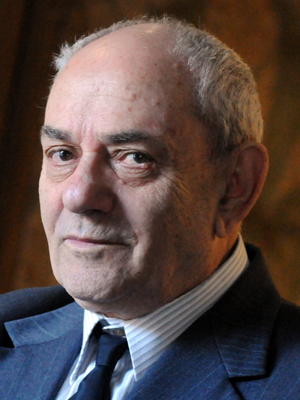
\includegraphics[height=0.34\textheight,keepaspectratio]{images/Vapnik.png}\\[-0.2em]
    {\scriptsize Vladimir Vapnik}
  \end{column}
  \begin{column}{0.45\textwidth}
    \centering
    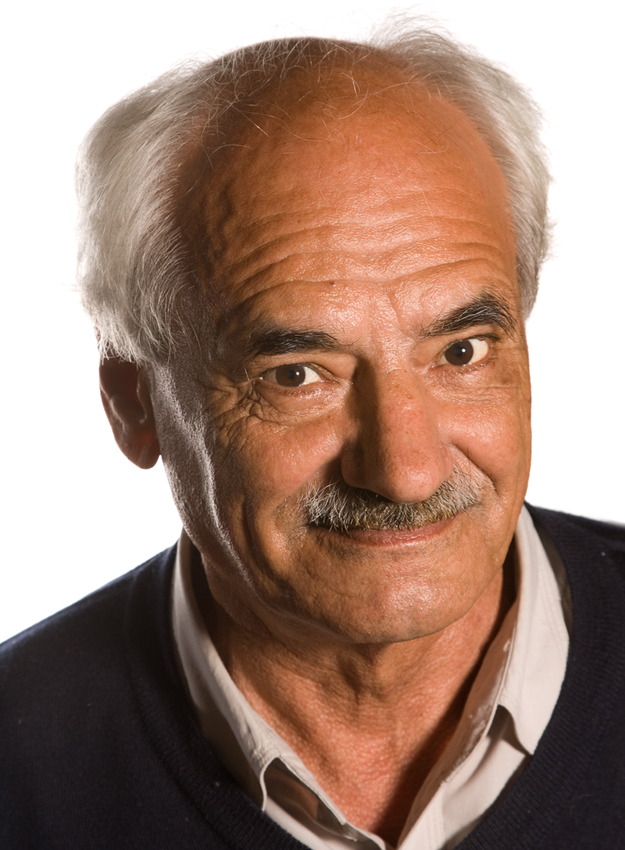
\includegraphics[height=0.34\textheight,keepaspectratio]{images/Chervonenkis.JPG}\\[-0.2em]
    {\scriptsize Alexey Chervonenkis}
  \end{column}
\end{columns}
\end{frame}

\begin{frame}{Simetrización}
Como no podemos calcular directamente $\mathcal{R}$, desearíamos acotar
la ecuación
\[
\sup_{f \in \mathcal{F}} |\mathcal{R}(f) - \mathcal{R}_{\text{emp}}(f)|
\]

por una cantidad que dependa de valores empíricos en su totalidad.\\

\bigskip
\pause
Vamos a necesitar una muestra fantasma.
\begin{center}
  
\includegraphics[width=0.50\textwidth]{images/casper.png}
\end{center}

\end{frame}

\begin{frame}
  \begin{block}{Lema de Simetrización}
    \large
 Sea $\mathcal{F}$ el espacio de funciones definido por un algoritmo de aprendizaje. Sean
$(X_i,Y_i)_{i=1,\dots, m}$, $(X_i',Y_i')_{i=1,\dots, m}$ muestras aleatorias iid. Dada $f \in\mathcal{F}$,
sean $\mathcal{R}(f)$ su riesgo, $\mathcal{R}_{emp}(f)$ su riesgo empírico sobre la primera muestra y
$\mathcal{R}'_{emp}(f)$ el riesgo sobre la segunda. Entonces, para cualquier $\varepsilon > 0$ tal que $m \geq \frac{2}{\varepsilon^2}$,
se cumple que

\[
P\left(\sup_{f \in \mathcal{F}} |\mathcal{R}(f) - \mathcal{R}_{\text{emp}}(f)| >
\varepsilon \right) \leq 2P\left(\sup_{f \in \mathcal{F}} |\mathcal{R}_{\text{emp}}(f) - \mathcal{R}'_{\text{emp}}(f)| > \frac{\varepsilon}{2}\right).
\]
  \end{block}
\bigskip
Este lema  nos permite trabajar
con eventos que dependen únicamente de las muestras observadas.
\end{frame}

\begin{frame}{Fragmentación}
Notemos que, incluso si \(\mathcal{F}\) contiene un número infinito de funciones,
las diferentes formas en que estas pueden clasificar un conjunto de entrenamiento de \(n\) puntos de muestra
es finita.\\
\pause
\bigskip
En efecto, para cualquier punto de entrenamiento dado en la muestra, una función puede tomar solo los valores
\(-1\) o \(+1\).

\begin{center}
  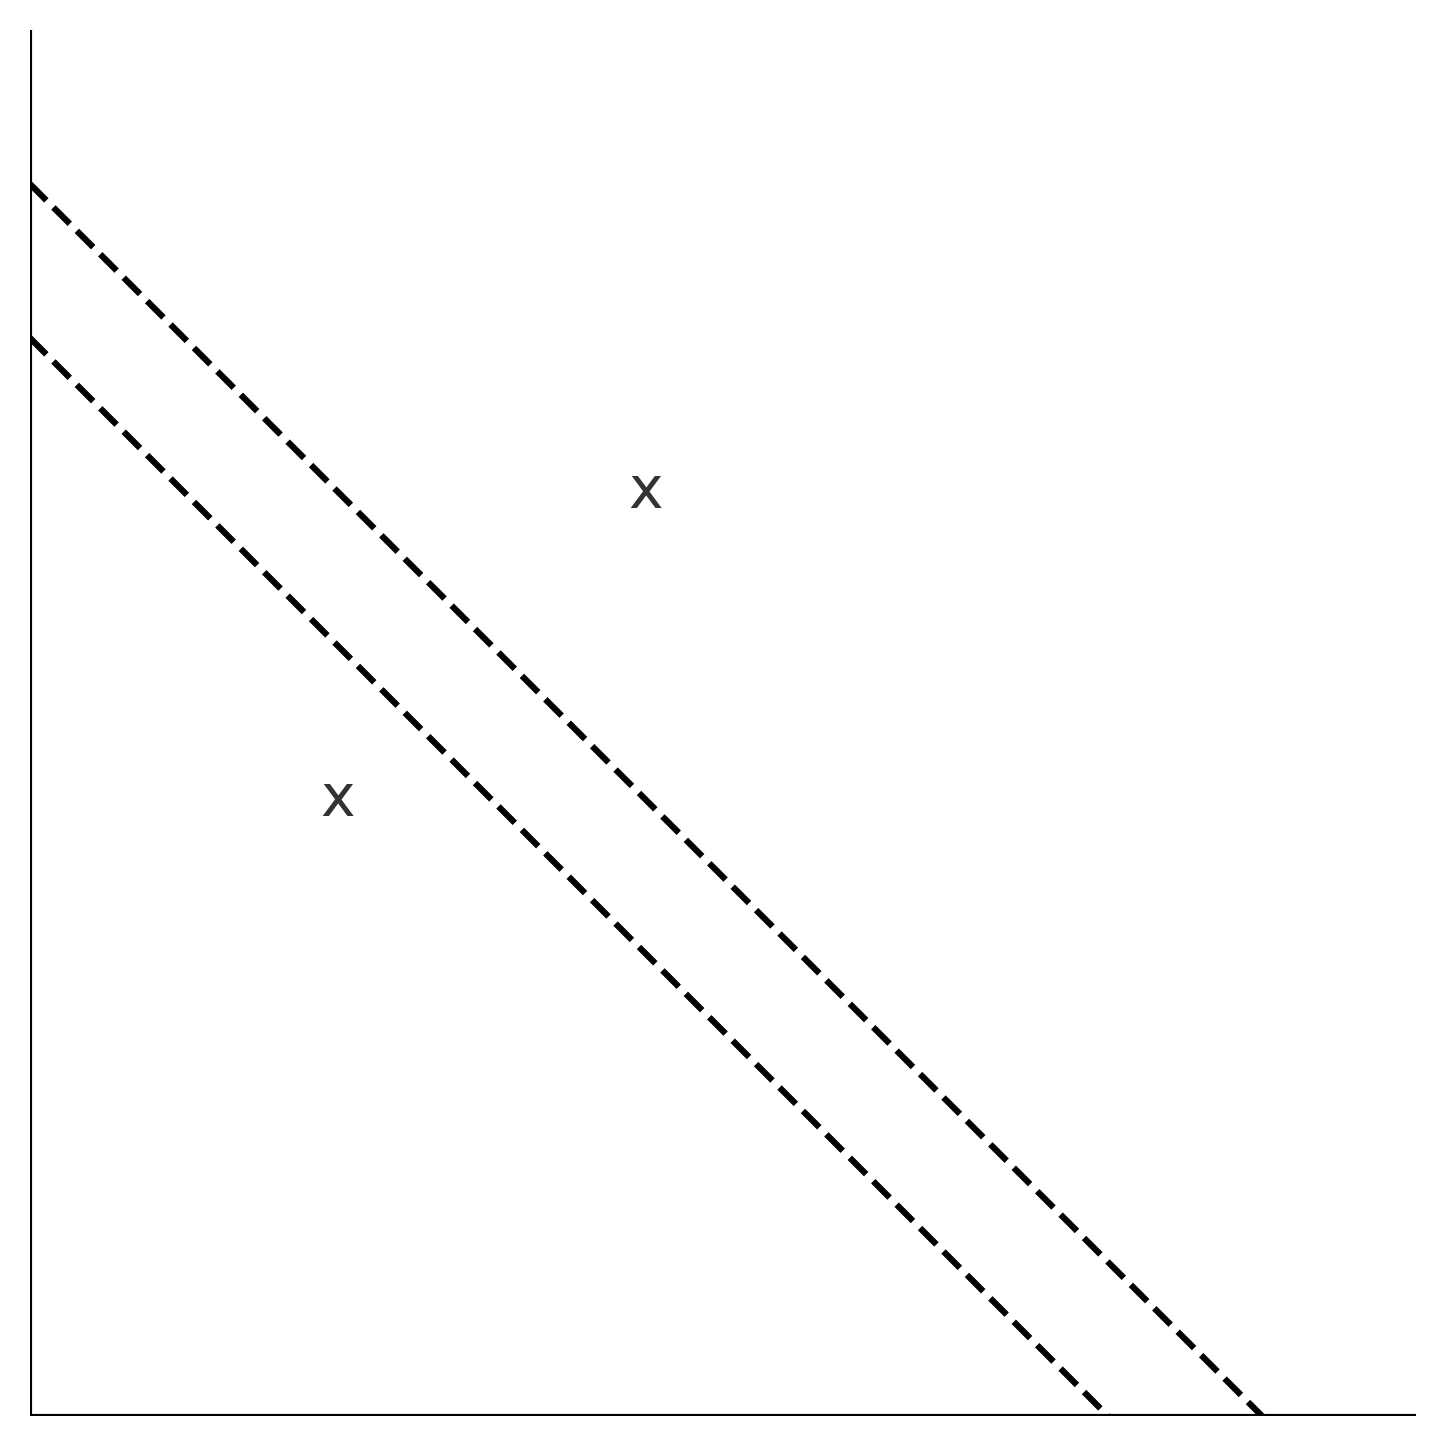
\includegraphics[width=\linewidth,height=0.48\textheight,keepaspectratio]{images/8.png}

  {\scriptsize\textcolor{gray}{Dos funciones que separan de igual manera a un par de puntos.}}
\end{center}

\end{frame}


\begin{frame}{Fragmentación}

      \begin{block}{Definición}
        Sean \(\mathcal{F}\) una clase de funciones y sea \(Z_n\) un conjunto de \(n\) puntos etiquetados, donde
        \[
        Z_n := \{(X_1, Y_1), \dots, (X_n, Y_n)\}.
        \]
        Definimos la relación \(\sim\) sobre \(\mathcal{F}\):
        \[
        f_1 \sim f_2 \quad \text{si} \quad f_1(X_i) = f_2(X_i) \quad \forall i = 1, \dots, n.
        \]
      \end{block}
\pause
\bigskip
      \begin{block}{Observación}
        La relación \(\sim\) es una relación de equivalencia sobre \(\mathcal{F}\).
      Luego, para una muestra fija, define una partición sobre \(\mathcal{F}\).
      \end{block}

\end{frame}

% \begin{frame}{Fragmentación}
%   En una muestra de \(n\) puntos \(\{X_1, \dots, X_n\}\), una función puede actuar de, como
% máximo, \(2^n\) formas diferentes.\\
% \bigskip
%  Así, las únicas funciones que
% necesitamos considerar para calcular el supremo son las \(2^{n}\) funciones que podemos obtener en la muestra
% original y la muestra fantasma juntas. Por lo tanto, podemos reemplazar el supremo sobre \(f \in \mathcal{F}\) por el
% supremo sobre una clase finita de funciones con como máximo \(2^{n}\) funciones
% \end{frame}


\begin{frame}{Fragmentación}
\begin{block}{Definición}
    Definimos el \textbf{conjunto de fragmentación} \(\mathcal{F}_{Z_n}\) a cualquier conjunto de representantes de \(\mathcal{F}\)
    bajo la relación de equivalencia \(\sim\) para la muestra $Z_n$.
\end{block}
\pause
\bigskip
Consideremos el espacio $\mathbb{R}^2$ y sea $\mathcal{F}=\{f: f(x)= \alpha x + \beta; \; \alpha, \beta\in\mathbb{R}\}$, el espacio
de funciones lineales.

  \begin{figure}[ht]
      \centering
    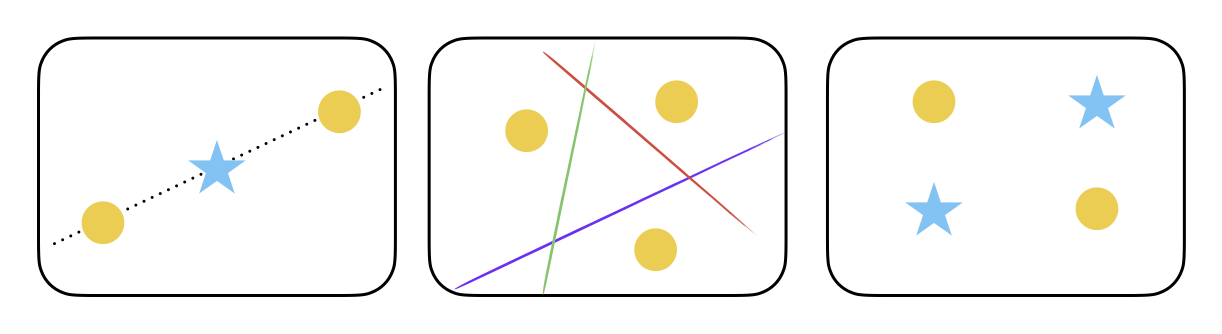
\includegraphics[width=0.8\textwidth]{images/linear fragmentation.png}
\end{figure}
\end{frame}

\begin{frame}{Fragmentación}

\begin{block}{Definición}
  \large
    Dado un espacio muestral \(X\) y una muestra \textbf{cualquiera} de tamaño \(n\), denotada por
    \[
    Z_n := \{(X_1, Y_1), \dots, (X_n, Y_n)\},
    \]
    definimos el
    \textbf{coeficiente de fragmentación} del espacio funcional $\mathcal{F}$ como:

    \[
    \mathcal{N}(\mathcal{F}, n) = \max_{Z_n} \{|\mathcal{F}_{Z_n}|\} = \max_{\{X_1, \dots, X_n\}}\{|\mathcal{F}_{\{X_1, \dots, X_n\}}| \mid X_1, \dots, X_n \in X\}.
    \]
\end{block}
\pause
\bigskip
  \begin{block}{Definición}
    Si \(\mathcal{N}(\mathcal{F}, n) = 2^n\), existe al menos una muestra de tamaño \(n\) que puede ser separada
de todas las formas posibles por funciones en \(\mathcal{F}\). En este caso, decimos que la clase de funciones
\(\mathcal{F}\) \textit{fragmenta} al conjunto de \(n\) puntos.
  \end{block}

\end{frame}

% \begin{frame}{Fragmentación}
%   $\mathcal{N}(\mathcal{F}, n)$ es el número máximo de formas en las que \(\mathcal{F}\) puede separar en dos clases a una muestra
%   de tamaño $n$ de $X$.\\
% \pause
% \bigskip
%   Esto no implica que \(\mathcal{F}\) pueda separar a \textbf{todas} las muestras de tamaño \(n\) de esta manera.\\
% \pause
% \bigskip
% En el caso de clasificación binaria, el mayor cardinal posible para un conjunto de fragmentación
% coincide con el cardinal del conjunto de partes de un conjunto de tamaño $n$.\\
% \pause
% \bigskip
% Si \(\mathcal{N}(\mathcal{F}, n) = 2^n\), existe al menos una muestra de tamaño \(n\) que puede ser separada
% de todas las formas posibles por funciones en \(\mathcal{F}\). En este caso, decimos que la clase de funciones
% \(\mathcal{F}\) \textit{fragmenta} al conjunto de \(n\) puntos.
% \end{frame}




\begin{frame}{El Coeficiente de Fragmentación y la Consistencia}
Consideremos una muestra de \(2n\) puntos. Volviendo al lema de simetrización, tenemos que
\[
\begin{aligned}
P\left(\sup_{f \in \mathcal{F}} |R(f) - R_{\text{emp}}(f)| > \varepsilon\right) &\leq
2P\left(\sup_{f \in \mathcal{F}} |R_{\text{emp}}(f) - R'_{\text{emp}}(f)| > \frac{\varepsilon}{2}\right)\\
\pause& = 2P\left(\sup_{f \in \mathcal{F}_{Z_{2n}}} |R_{\text{emp}}(f) - R'_{\text{emp}}(f)| > \frac{\varepsilon}{2}\right)\\
\pause& \leq 2  \mathcal{N}(\mathcal{F}, n)\cdot \exp\left(\frac{-n\varepsilon^2}{4}\right).
\end{aligned}
\]
\end{frame}


% \begin{frame}{El Coeficiente de Fragmentación y la Consistencia}


% Tomemos $\mathcal{F}_{all}$, el espacio de todos los clasificadores posibles. \\
%  \pause
%  \bigskip
% En este caso, $\mathcal{N}(\mathcal{F}_{all}, n)=2^{2n}$,
% pues cualquier muestra de $2n$ puntos puede ser separada de $2^{2n}$ formas posibles. \pause Entonces, la cota de convergencia uniforme para este espacio
% es:

% \[
% \begin{aligned}
% P\left(\sup_{f \in \mathcal{F}_{all}} |R(f) - R_{\text{emp}}(f)| > \varepsilon \right)
% &\leq 2\cdot 2^{2n} \exp\left(-\frac{n\varepsilon^2}{4}\right) \\
% \pause&= 2\exp\left(n\left( 2\log(2) - \frac{n\varepsilon^2}{4}\right)\right).
% \end{aligned}
% \]

% \end{frame}

% \begin{frame}
%   Que es una expresión que no tiende a $0$ cuando $n$ tiende a infinito. \\
%   \pause
%   \bigskip
%   Esto no significa que podamos
% concluir que la MRE no es consistente con respecto a $\mathcal{F}_{all}$.\\
% \pause
% \bigskip
% Pero si podemos dar el siguiente resultado:
% \begin{block}{Teorema}
%     La minimización del riesgo empírico es consistente con respecto a un espacio de funciones $\mathcal{F}$ si y solo si
%     \[
%     \frac{\log\left(\mathcal{N}(\mathcal{F}, n)\right)}{n} \rightarrow 0 \qquad \text{cuando } n \to \infty.
%     \]
% \end{block}
% \end{frame}

\begin{frame}{El Coeficiente de Fragmentación y la Consistencia}
  \begin{block}{Teorema}
    \large
    La minimización del riesgo empírico es consistente con respecto a un espacio de funciones $\mathcal{F}$ si y solo si
    \[
    \frac{\log\left(\mathcal{N}(\mathcal{F}, n)\right)}{n} \rightarrow 0 \qquad \text{cuando } n \to \infty.
    \]
\end{block}
\pause
  \begin{block}{Corolario 1}
    Si $\mathcal{N}(\mathcal{F}, n)$ es polinómica, entonces la minimización del riesgo empírico es consistente con respecto a $\mathcal{F}$.\\
\end{block}
\pause
\begin{block}{Corolario 2}
    Si $\mathcal{N}(\mathcal{F}, n)=2^n$, entonces la minimización del riesgo empírico no es consistente con respecto a $\mathcal{F}$. En
    particular, no es consistente con respecto al espacio de todas los clasificadores posibles $\mathcal{F}_{all}$.
\end{block}
\end{frame}

\begin{frame}{La dimensión VC}
\begin{block}{Definición}
  \large
    La dimensión VC de una clase de funciones \(\mathcal{F}\) es el tamaño máximo de una muestra que puede ser fragmentada por \(\mathcal{F}\), es decir:
    \[
    \text{VC}(\mathcal{F}) = \max \{n \in \mathbb{N} \mid \mathcal{N}(\mathcal{F}, n) = 2^n\}.
    \]
    Si no existe tal máximo, definimos \(\text{VC}(\mathcal{F}) = \infty\).
\end{block}
\pause
\begin{block}{Teorema}
  La dimensión VC del espacio de funciones lineales en \(\mathbb{R}^2\) es \(3\).
\end{block}

\pause


\begin{block}{Teorema}
  La dimensión VC del espacio de funciones lineales en \(\mathbb{R}^d\) es \(d+1\).
\end{block}

\end{frame}

\begin{frame}{La dimensión VC}
  \begin{block}{Lema}
    \Large
      Sea $\mathcal{F}$ una clase de funciones con dimensión VC finita. Entonces
    \[
    \mathcal{N}(\mathcal{F}, n) \leq \sum_{i=0}^{\text{VC}(\mathcal{F})} \binom{n}{i} , \qquad \forall n \in \mathbb{N}.
    \]
    En particular, para $n\geq \text{VC}(\mathcal{F})$ se tiene que
    \[
    \mathcal{N}(\mathcal{F}, n) \leq \left(\frac{e\cdot n}{\text{VC}(\mathcal{F})}\right)^{\text{VC}(\mathcal{F})}.
    \]
    \end{block}
\end{frame}


\begin{frame}{La dimensión VC}
Si \( n \geq \text{VC}(\mathcal{F}) \),
el coeficiente de fragmentación se comporta como una función polinómica del tamaño de la muestra \( n \).\\
\bigskip
\pause
Por los resultados de la sección anterior, esto implica la consistencia de la minimización del riesgo empírico.\\
\bigskip
\pause
Si la dimensión VC es infinita, para cada \( n \) existe alguna muestra que puede ser fragmentada por \(\mathcal{F}\).\\

\pause
\bigskip

  \begin{block}{Teorema}
    \Large
    La minimización del riesgo empírico es consistente con respecto a una clase de funciones \(\mathcal{F}\) si y solo si
    la dimensión VC de \(\mathcal{F}\) es finita.
\end{block}

\end{frame}

\rotuloslide{05}{Límites y panorama actual}{No hay almuerzos gratis y la paradoja moderna}

\begin{frame}{No hay almuerzos gratis}
  \large
¿Cuál de todos los clasificadores consistentes
es \textit{el mejor} clasificador?  \\
\bigskip
\pause
¿Existe un clasificador universalmente bueno?\\

\bigskip
\pause
No solamente no existe un clasificador universalmente bueno, sino que, en promedio sobre todas las distribuciones
posibles, todos los clasificadores son equivalentes.


\end{frame}
\begin{frame}
  \Large
\begin{block}{El Teorema de la chancha y los veinte}
    Sea \(\varepsilon > 0\). Para cualquier entero \(n\) y cualquier
regla de clasificación \(f_n\), existe una distribución \(P(X, Y)\) con riesgo bayesiano
\(\mathcal{R}(f_{Bayes}) = 0\) tal que:

\[
\mathbb{E}[\ell(X,Y,f_n)] \geq \frac{1}{2} - \varepsilon.
\]
\end{block}


\end{frame}

\begin{frame}{La Paradoja Moderna}



      \vspace{0.5em}
      \begin{alertblock}{ }
         En la práctica, los modelos de aprendizaje profundo modernos son \textbf{extremadamente sobreparametrizados}.
         Por ejemplo,
        GPT-4: ${\sim}1.8$\,T parámetros, $n \ll \text{parámetros}$.
        Las cotas VC serían \textbf{astronómicamente grandes}
        \centering\alert{…y sin embargo, generalizan.}
      \end{alertblock}
\pause
      \centering
      %% f(x) = 0.08 + 0.80*exp(-0.55x) + 0.58*exp(-3.5*(x-5.5)^2)
      %% Valores clave:  x=0 → 0.88,  x=4 → 0.17,  x=5.5 → 0.70 (pico),
      %%                 x=7 → 0.09,  x=10 → 0.08
      %% Ambos trazos usan la MISMA función → curva continua
      \begin{tikzpicture}
        \begin{axis}[
            width=6.8cm, height=5.0cm,
            axis lines=left,
            xlabel={complejidad del modelo},
            ylabel={error de generalización},
            xlabel style={font=\scriptsize},
            ylabel style={font=\scriptsize},
            xmin=0, xmax=10,
            ymin=0, ymax=1.0,
            xtick=\empty, ytick=\empty,
            clip=false,
            legend style={font=\scriptsize, row sep=-2pt,
                          at={(0.98,0.98)}, anchor=north east},
          ]
          %% Régimen clásico (sesgo–varianza): x de 0 a 5.5
          \addplot[very thick, uncoBlue, domain=0.05:5.5, samples=200]
            {0.08 + 0.80*exp(-0.55*x) + 0.58*exp(-3.5*(x-5.5)^2)};
          \addlegendentry{\scriptsize teoría clásica};
          %% Régimen moderno (doble descenso): x de 5.5 a 10
          \addplot[very thick, red, dashed, domain=5.5:10, samples=200]
            {0.08 + 0.80*exp(-0.55*x) + 0.58*exp(-3.5*(x-5.5)^2)};
          \addlegendentry{\scriptsize DL moderno};
          %% Línea vertical en el umbral de interpolación
          \draw[dotted, gray!70, thick]
            (axis cs:5.5, 0) -- (axis cs:5.5, 0.72);
          \node[font=\tiny, gray, rotate=90] at (axis cs:5.18, 0.37)
            {umbral interp.};
          %% Etiqueta mínimo clásico
          \node[font=\tiny, uncoBlue, align=center] at (axis cs:2.2, 0.38)
            {sesgo-\\varianza};
          %% Etiqueta doble descenso
          \node[font=\tiny, red!80, align=center] at (axis cs:8.3, 0.30)
            {doble\\descenso};
        \end{axis}
      \end{tikzpicture}

      {\scriptsize\textcolor{gray}{Fenómeno de ``doble descenso'':
      el error \emph{vuelve a bajar} tras la sobreparametrización.}}

\end{frame}


% \begin{frame}
%   \begin{block}{ }
%   En aquel Imperio, el Arte de la Cartografía logró tal Perfección que el mapa de una sola Provincia ocupaba toda una Ciudad, 
%   y el mapa del Imperio, toda una Provincia. Con el tiempo, estos Mapas Desmesurados no satisficieron y los Colegios de Cartógrafos 
%   levantaron un Mapa del Imperio, que tenía el tamaño del Imperio y coincidía puntualmente con él.\\
% \bigskip
% Menos Adictas al Estudio de la Cartografía, las Generaciones Siguientes entendieron que ese dilatado Mapa era Inútil y 
% o sin Impiedad lo entregaron a las Inclemencias del Sol y los Inviernos. En los desiertos del Oeste perduran despedazadas 
% Ruinas del Mapa, habitadas por Animales y por Mendigos; en todo el País no hay otra reliquia de las Disciplinas Geográficas.
% \bigskip
% Suárez Miranda, Viajes de Varones Prudentes, Libro Cuarto, Cap. XLV, Lérida, 1658.
%         \vspace{0.5em}
%         \begin{flushright}
%           \normalfont\scriptsize
%           ---~Jorge Luis Borges,\\
%           \textit{Del Rigor en la Ciencia} (1946)
%         \end{flushright}
%   \end{block}
% \end{frame}



% % ==============================================================================
% % SLIDE 2: El quiebre de la teoría clásica
% % ==============================================================================
% \begin{frame}{El quiebre de la teoría clásica}
%     \begin{columns}[c]
%         \begin{column}{0.55\textwidth}
%             \centering
%             \begin{minipage}{\textwidth}
%                 \textcolor{accentblue}{\textbf{Complejidad vs. generalización}}
%                 \vspace{0.3cm}
%                 \begin{itemize}
%                     \item \textbf{Cotas vacías:} la teoría VC implica que, cuando el número de parámetros excede ampliamente al tamaño muestral ($d \gg n$), la brecha de generalización deja de ser informativa ($>100\%$).
%                     \vspace{0.2cm}
%                     \item \textbf{Capacidad casi infinita:} los LLM modernos tienen cientos de miles de millones de parámetros; en principio podrían fragmentar cualquier conjunto de datos, pero evitan el sobreajuste catastrófico.
%                     \vspace{0.2cm}
%                     \item \textbf{Paradoja estructural:} la estrategia clásica de restringir la capacidad de $\mathcal{F}$ para forzar convergencia uniforme queda tensionada por las arquitecturas modernas.
%                 \end{itemize}
%             \end{minipage}
%         \end{column}
        
%         \begin{column}{0.4\textwidth}
%             \begin{block}{Cota clásica de generalización}
%                 \vspace{0.2cm}
%                 \[
%                 R(f) \le R_n(f) + \sqrt{\frac{d \left(\ln \frac{2n}{d} + 1\right) + \ln \frac{4}{\delta}}{n}}
%                 \]
%                 \vspace{0.1cm}
%                 \centering \scriptsize \textcolor{gray}{Donde $d = \text{VC}(\mathcal{F})$ y $n = \text{tamaño muestral}$}
%             \end{block}
%             \vspace{0.3cm}
%             \begin{center}
%                 \scriptsize \textcolor{red!70!black}{\textbf{Problema:}} si $d \gg n$, el término radical explota y la cota se vuelve inútil para modelos profundos.
%             \end{center}
%         \end{column}
%     \end{columns}
% \end{frame}

% ==============================================================================
% SLIDE 3: Reconciliar teoría y realidad
% ==============================================================================
\begin{frame}{El rol de la Matemática en la era de la IA}
    \begin{columns}[t]
        \begin{column}{0.31\textwidth}
            \begin{block}{1. Doble descenso}
                \small
                La sobreparametrización permite que la optimización elija 
                \textbf{funciones más regulares} pese a la enorme capacidad disponible.
            \end{block}
        \end{column}
        \pause
        \begin{column}{0.31\textwidth}
            \begin{block}{2. Sesgo implícito}
                \small
                El espacio $\mathcal{F}$ es nominalmente enorme, pero la optimización (SGD) actúa como un \textbf{regularizador implícito}.
                \vspace{0.2cm}
               \end{block}
        \end{column}
        \pause
        \begin{column}{0.31\textwidth}
            \begin{block}{3. Geometría de los datos}
                \small
               Los datos de texto e imágenes se concentran en \textbf{variedades} de baja dimensión,
               por lo que la capacidad efectiva de $\mathcal{F}$ es mucho menor que la dimensión VC.
            \end{block}
        \end{column}
    \end{columns}
    \pause
    \vspace{0.6cm}
    \begin{beamercolorbox}[wd=\textwidth, rounded=true, center, sep=8pt]{lightbg}
        \textcolor{accentblue}{\textbf{El desarollo de una teoría robusta para explicar la generalización en los LLMs es un problema abierto.}
        } \pause \\
        La humanidad necesita que los matemáticos contribuyan a entender y \textit{desarmar} la IA.
      \end{beamercolorbox}

\end{frame}

% % ==============================================================================
% % SLIDE 4: Hoja de ruta para matemáticos
% % ==============================================================================
% \begin{frame}{Hoja de ruta para matemáticos}
%     \begin{columns}[T]
%         \begin{column}{0.45\textwidth}
%             \small
%             \textcolor{accentblue}{\textbf{Fronteras teóricas clave}}
%             \vspace{0.15cm}
%             \begin{itemize}
%                 \setlength{\itemsep}{0.15cm}
%                 \item Las herramientas tradicionales tienen dificultades con parametrizaciones altamente sobreparametrizadas.
%                 \item El estado del arte exige formular preguntas estadísticas como problemas geométricos y algebraicos.
%                 \item Tender puentes entre las trayectorias continuas de la optimización y la mecánica discreta de la complejidad muestral.
%             \end{itemize}
%         \end{column}
        
%         \begin{column}{0.5\textwidth}
%             \setbeamercolor{block title}{bg=primaryblue, fg=white}
%             \begin{block}{Teoría singular del aprendizaje (SLT)}
%                 \scriptsize
%                 Las parametrizaciones de redes neuronales son altamente singulares (no identificables). La SLT usa geometría algebraica para estudiar la generalización mediante el \textbf{Real Log Canonical Threshold (RLCT)}, que cuantifica la complejidad geométrica local de los valles singulares.
%             \end{block}
            
%             \begin{block}{Análisis de trayectorias estocásticas}
%                 \scriptsize
%                 Modelar las trayectorias discretas de SGD como \textbf{ecuaciones diferenciales estocásticas (SDEs)} en tiempo continuo. El objetivo es vincular formalmente las trayectorias de optimización con cuencas de mínimos planas y buena generalización.
%             \end{block}
            
%             \begin{block}{Más allá del cuello de botella NTK}
%                 \scriptsize
%                 Superar los límites estáticos de ancho infinito (\textit{lazy training}) para formalizar el verdadero \textbf{aprendizaje de representaciones}, donde el kernel reproductor asociado evoluciona dinámicamente con los datos.
%             \end{block}
%         \end{column}
%     \end{columns}
% \end{frame}





% ─────────────────────────────────────────────────────────────
% ─────────────────────────────────────────────────────────────
% ─────────────────────────────────────────────────────────────
% ─────────────────────────────────────────────────────────────
% ─────────────────────────────────────────────────────────────
% ─────────────────────────────────────────────────────────────
% ─────────────────────────────────────────────────────────────
% ─────────────────────────────────────────────────────────────
% ─────────────────────────────────────────────────────────────
% ─────────────────────────────────────────────────────────────
% ─────────────────────────────────────────────────────────────
% ─────────────────────────────────────────────────────────────
% ─────────────────────────────────────────────────────────────
% ─────────────────────────────────────────────────────────────




% % ─────────────────────────────────────────────────────────────
% % BLOQUE 2: LA TRAMPA DE LA LIBERTAD
% % ─────────────────────────────────────────────────────────────

% %--------------------------------------------------------------
% % DIAPOSITIVA 6 — EL ATAJO EMPÍRICO
% %--------------------------------------------------------------
% \begin{frame}{Riesgo Empírico}
%   \begin{columns}[T]

%     %% — Columna izquierda: la fórmula y su origen
%     \begin{column}{0.54\textwidth}
%       \textbf{Riesgo Empírico} (lo que \textit{sí} podemos calcular):
%       \[
%         \mathcal{R}_{\mathrm{emp}}(f)
%         \;:=\;
%         \frac{1}{n}\sum_{i=1}^{n}\ell\bigl(X_i,\,Y_i,\,f(X_i)\bigr)
%       \]

%       \vspace{0.5em}
%       \textbf{Principio ERM} (Minimización del Riesgo Empírico):
%       \[
%         f_n \;:=\; \arg\min_{f \in \mathcal{F}}\;\mathcal{R}_{\mathrm{emp}}(f)
%       \]

%       \vspace{0.4em}
%       {\small La motivación proviene de la \textbf{Ley de los Grandes Números}:}
%       \[
%         \frac{1}{n}\sum_{i=1}^{n}\xi_i
%         \;\xrightarrow{\;n\to\infty\;}
%         \mathbb{E}[\xi]
%         \qquad (\xi_i \;\text{i.i.d.})
%       \]
%     \end{column}

%     %% — Columna derecha: por qué parece funcionar y la advertencia
%     \begin{column}{0.44\textwidth}
%       \begin{block}{La promesa}
%         Para $f$ \textbf{fija}, la LGN garantiza:
%         \[
%           \mathcal{R}_{\mathrm{emp}}(f)
%           \;\xrightarrow{\;n\to\infty\;}
%           \mathcal{R}(f)
%         \]
%         Más datos $\;\Rightarrow\;$ mejor estimación.
%       \end{block}

%       \vspace{0.7em}

%       \begin{alertblock}{La trampa oculta}
%         Nuestra $f_n$ \textbf{depende de los datos}.\\[0.3em]
%         La LGN aplica a funciones \textit{fijas},
%         no a funciones que cambian con la muestra.
%       \end{alertblock}
%     \end{column}

%   \end{columns}
% \end{frame}

% %--------------------------------------------------------------
% % DIAPOSITIVA 7 — EL COLAPSO DE LA MEMORIZACIÓN
% %--------------------------------------------------------------
% \begin{frame}{El Colapso de la Memorización: $\mathcal{F}_{\mathrm{all}}$}
%   \begin{columns}[T]

%     %% — Columna izquierda: el clasificador tramposo
%     \begin{column}{0.50\textwidth}
%       \textbf{El clasificador ``tramposo''}
%       (búsqueda irrestricta en $\mathcal{F}_{\mathrm{all}}$):
%       \[
%         f_n(X) \;:=\;
%         \begin{cases}
%           Y_i & \text{si } X = X_i \text{ para algún } i \\
%           +1  & \text{en otro caso}
%         \end{cases}
%       \]

%       \vspace{0.6em}
%       \begin{itemize}
%         \setlength{\itemsep}{0.45em}
%         \item $\mathcal{R}_{\mathrm{emp}}(f_n) = 0$ \hfill \textcolor{green!60!black}{(perfecto en train)}
%         \item $\mathcal{R}(f_n) = \tfrac{1}{2}$ \hfill \alert{(moneda al aire en test)}
%       \end{itemize}

%       \vspace{0.6em}
%       \begin{alertblock}{Diagnóstico}
%         \textbf{Sobreajuste catastrófico.}\\
%         El algoritmo aprendió los datos, no la regla.
%       \end{alertblock}
%     \end{column}

%     %% — Columna derecha: figura intuitiva
%     \begin{column}{0.48\textwidth}
%       \centering
%       \begin{tikzpicture}[scale=0.92]
%         \begin{axis}[
%             width=6.5cm, height=5.5cm,
%             axis lines=center,
%             xlabel=$x$, ylabel=$y$,
%             xlabel style={font=\small, at={(axis description cs:1,0)}, anchor=west},
%             ylabel style={font=\small, at={(axis description cs:0,1)}, anchor=south},
%             xmin=-0.3, xmax=5.5,
%             ymin=-0.5, ymax=2.0,
%             xtick=\empty, ytick=\empty,
%             clip=false,
%           ]
%           %% Puntos de entrenamiento clase +1
%           \addplot[only marks, mark=*, mark size=3pt, uncoBlue]
%             coordinates{(0.8,1.0)(1.5,1.0)(2.8,1.0)(4.2,1.0)};
%           %% Puntos de entrenamiento clase -1
%           \addplot[only marks, mark=square*, mark size=3pt, red]
%             coordinates{(1.1,0.0)(2.2,0.0)(3.5,0.0)(4.8,0.0)};
%           %% Punto de prueba nuevo (no visto)
%           \addplot[only marks, mark=triangle*, mark size=4pt, orange]
%             coordinates{(3.0,0.5)};
%           %% Etiquetas
%           \node[font=\scriptsize, uncoBlue, above] at (axis cs:0.8,1.0) {$+1$};
%           \node[font=\scriptsize, uncoBlue, above] at (axis cs:1.5,1.0) {$+1$};
%           \node[font=\scriptsize, uncoBlue, above] at (axis cs:2.8,1.0) {$+1$};
%           \node[font=\scriptsize, uncoBlue, above] at (axis cs:4.2,1.0) {$+1$};
%           \node[font=\scriptsize, red, below]  at (axis cs:1.1,0.0) {$-1$};
%           \node[font=\scriptsize, red, below]  at (axis cs:2.2,0.0) {$-1$};
%           \node[font=\scriptsize, red, below]  at (axis cs:3.5,0.0) {$-1$};
%           \node[font=\scriptsize, red, below]  at (axis cs:4.8,0.0) {$-1$};
%           %% Punto nuevo con predicción errónea
%           \node[font=\scriptsize, orange, right] at (axis cs:3.0,0.5)
%             {\;$x_{\mathrm{nuevo}}$\;\alert{$\hat{y}=+1$??}};
%         \end{axis}
%       \end{tikzpicture}

%       \vspace{0.2em}
%       {\scriptsize\textcolor{gray}{$f_n$ memoriza el train; ignora el test.}}
%     \end{column}

%   \end{columns}
% \end{frame}

% %--------------------------------------------------------------
% % DIAPOSITIVA 8 — EL DILEMA DE LA COMPLEJIDAD
% %--------------------------------------------------------------
% \begin{frame}{El Dilema de la Complejidad}
%   \begin{columns}[T]

%     %% — Columna izquierda: la ecuación de descomposición
%     \begin{column}{0.50\textwidth}
%       \textbf{Descomposición del exceso de riesgo:}
%       \[
%         \underbrace{\mathcal{R}(f_n) - \mathcal{R}(f_{\mathrm{Bayes}})}_{\text{lo que queremos reducir}}
%       \]
%       \[
%         =\;
%         \underbrace{\mathcal{R}(f_n) - \mathcal{R}(f_{\mathcal{F}})}_{\textcolor{red}{\text{error de estimación}}}
%         \;+\;
%         \underbrace{\mathcal{R}(f_{\mathcal{F}}) - \mathcal{R}(f_{\mathrm{Bayes}})}_{\textcolor{uncoBlue}{\text{error de aproximación}}}
%       \]

%       \vspace{0.6em}
%       \begin{itemize}
%         \setlength{\itemsep}{0.4em}
%         \item \textcolor{uncoBlue}{\textbf{Aprox.:}} $\mathcal{F}$ pequeño $\Rightarrow$ alto \textcolor{uncoBlue}{sesgo} (subajuste).
%         \item \textcolor{red}{\textbf{Estim.:}} $\mathcal{F}$ grande $\Rightarrow$ alta \textcolor{red}{varianza} (sobreajuste).
%       \end{itemize}
%     \end{column}

%     %% — Columna derecha: figura sesgo-varianza (Figura 2.3)
%     \begin{column}{0.48\textwidth}
%       \centering
%       \begin{tikzpicture}
%         \begin{axis}[
%             width=6.8cm, height=5.2cm,
%             axis lines=left,
%             xlabel={complejidad de $\mathcal{F}$},
%             ylabel={error},
%             xlabel style={font=\scriptsize},
%             ylabel style={font=\scriptsize},
%             xmin=0, xmax=6,
%             ymin=0, ymax=3.2,
%             xtick=\empty, ytick=\empty,
%             clip=false,
%             legend pos=north east,
%             legend style={font=\scriptsize, row sep=-2pt},
%           ]
%           %% Error de aproximación (decreasing)
%           \addplot[thick, uncoBlue, domain=0.2:5.8, samples=100]
%             {2.5*exp(-0.65*x) + 0.05};
%           \addlegendentry{\textcolor{uncoBlue}{aprox.}};
%           %% Error de estimación (increasing)
%           \addplot[thick, red, domain=0.2:5.8, samples=100]
%             {0.08*x^2 - 0.1*x + 0.15};
%           \addlegendentry{\textcolor{red}{estim.}};
%           %% Riesgo total (U-shaped)
%           \addplot[thick, black, domain=0.2:5.8, samples=100]
%             {2.5*exp(-0.65*x) + 0.08*x^2 - 0.1*x + 0.20};
%           \addlegendentry{riesgo total};
%           %% Mínimo óptimo (flecha)
%           \draw[dashed, gray] (axis cs:2.05,0) -- (axis cs:2.05,1.45);
%           \node[font=\scriptsize, gray, below] at (axis cs:2.05,0) {óptimo};
%         \end{axis}
%       \end{tikzpicture}

%       \vspace{0.1em}
%       {\scriptsize\textcolor{gray}{Inspirado en Figura 2.3 de la tesina.}}
%     \end{column}

%   \end{columns}
% \end{frame}

% %--------------------------------------------------------------
% % DIAPOSITIVA 9 — LA NECESIDAD DE UN SESGO (PUENTE A VC)
% %--------------------------------------------------------------
% \begin{frame}{La Necesidad de un Sesgo Inductivo}
%   \begin{columns}[T]

%     %% — Columna izquierda: la conclusión forzosa
%     \begin{column}{0.50\textwidth}
%       \begin{block}{Conclusión del bloque}
%         Para que ERM sea \textbf{consistente}, el espacio $\mathcal{F}$
%         debe ser \alert{suficientemente restringido}.
%       \end{block}

%       \vspace{0.7em}
%       \begin{itemize}
%         \setlength{\itemsep}{0.55em}
%         \item $\mathcal{F} = \mathcal{F}_{\mathrm{all}}$ \;\alert{$\Rightarrow$}\; inconsistencia garantizada.
%         \item $\mathcal{F}$ pequeño (e.g., funciones lineales)\;
%               \textcolor{green!60!black}{$\Rightarrow$}\; bajo error de estimación.
%         \item Todo aprendizaje exitoso impone un \textbf{sesgo inductivo}.
%       \end{itemize}

%       \vspace{0.7em}
%       {\small No existe conocimiento sin suposición. \\ La pregunta es cuál suposición elegir.}
%     \end{column}

%     %% — Columna derecha: la pregunta puente
%     \begin{column}{0.48\textwidth}
%       \begin{alertblock}{Pregunta puente}
%         ¿Cómo \textbf{medir formalmente} si un espacio
%         $\mathcal{F}$ es lo suficientemente ``restringido''
%         para que ERM no nos mienta?
%       \end{alertblock}

%       \vspace{0.8em}

%       \begin{tikzpicture}[scale=0.85]
%         %% Círculo grande: F_all
%         \draw[thick, uncoBlue!40, fill=uncoBlue!5]
%               (0,0) circle (2.1cm);
%         \node[font=\small, uncoBlue!70] at (0, 1.6) {$\mathcal{F}_{\mathrm{all}}$};
%         %% Círculo pequeño: F restringido
%         \draw[thick, uncoBlue, fill=uncoBlue!20]
%               (0.2,-0.1) circle (0.9cm);
%         \node[font=\small, uncoBlue] at (0.2,-0.1) {$\mathcal{F}$};
%         %% Punto f_Bayes fuera de F
%         \fill[red] (-1.2, 0.3) circle (3pt);
%         \node[font=\scriptsize, red, left] at (-1.2, 0.3) {$f_{\mathrm{Bayes}}$};
%         %% Flechas / etiqueta
%         \node[font=\scriptsize, gray] at (0, -2.6)
%           {Restringir $\Leftrightarrow$ controlar la capacidad};
%       \end{tikzpicture}

%       \vspace{0.4em}
%       \centering
%       \large $\;\longrightarrow\;$ \textbf{Teoría VC}
%     \end{column}

%   \end{columns}
% \end{frame}

% % ─────────────────────────────────────────────────────────────
% % BLOQUE 3: EL ANDAMIAJE FORMAL — TEORÍA VC
% % ─────────────────────────────────────────────────────────────

% %--------------------------------------------------------------
% % DIAPOSITIVA 10 — LA LEY QUE NOS QUEDÓ CHICA
% %--------------------------------------------------------------
% \begin{frame}{La Ley que nos Quedó Chica: Convergencia Uniforme}
%   \begin{columns}[T]

%     \begin{column}{0.52\textwidth}
%       \textbf{LGN para $f$ fija} (lo que ya teníamos):
%       \[
%         \mathcal{R}_{\mathrm{emp}}(f)
%         \;\xrightarrow{\;n\to\infty\;}
%         \mathcal{R}(f)
%         \qquad\textcolor{green!60!black}{\checkmark}
%       \]

%       \vspace{0.5em}
%       \textbf{Lo que realmente necesitamos:}
%       \[
%         \sup_{f\,\in\,\mathcal{F}}
%         \bigl|\mathcal{R}(f) - \mathcal{R}_{\mathrm{emp}}(f)\bigr|
%         \;\xrightarrow{\;n\to\infty\;} 0
%         \quad\alert{(?)}
%       \]
%       {\small Convergencia \textit{simultánea} para \textbf{todas} las $f\in\mathcal{F}$.}
%     \end{column}

%     \begin{column}{0.46\textwidth}
%       \begin{alertblock}{¿Por qué la LGN no alcanza?}
%         $f_n = \arg\min_{f\in\mathcal{F}}\mathcal{R}_{\mathrm{emp}}(f)$
%         \textbf{depende de los datos}.\\[0.3em]
%         La LGN aplica a funciones \textit{fijas}, no a funciones que cambian con la muestra.
%       \end{alertblock}

%       \vspace{0.5em}

%       \begin{block}{Lo que hay que probar}
%         \[
%           P\!\left(
%             \sup_{f\in\mathcal{F}}
%             \bigl|\mathcal{R}(f)-\mathcal{R}_{\mathrm{emp}}(f)\bigr|>\varepsilon
%           \right)
%           \xrightarrow{n\to\infty} 0
%         \]
%         para todo $\varepsilon > 0$.
%       \end{block}
%     \end{column}

%   \end{columns}
% \end{frame}

% %--------------------------------------------------------------
% % DIAPOSITIVA 11 — COEFICIENTE DE FRAGMENTACIÓN
% %--------------------------------------------------------------
% \begin{frame}{Geometría de la Capacidad: Coeficiente de Fragmentación}
%   \begin{columns}[T]

%     \begin{column}{0.50\textwidth}
%       \begin{block}{Coeficiente de fragmentación}
%         \[
%           N(\mathcal{F},\,n) \;:=\;
%           \max_{x_1,\ldots,x_n\in\mathcal{X}}
%           \bigl|\bigl\{(f(x_1),\ldots,f(x_n)):f\in\mathcal{F}\bigr\}\bigr|
%         \]
%       \end{block}

%       \vspace{0.5em}
%       \begin{itemize}
%         \setlength{\itemsep}{0.45em}
%         \item Reduce $\mathcal{F}$ (infinito) a un conteo \textbf{combinatorio finito}.
%         \item $N(\mathcal{F},n) \leq 2^n$ siempre; la igualdad = \textit{fragmentación completa}.
%         \item Clasificadores lineales en $\mathbb{R}^2$:
%           \[N(\mathcal{F},\,3) = 8 = 2^3 \quad\textcolor{green!60!black}{\checkmark}\]
%       \end{itemize}
%     \end{column}

%     \begin{column}{0.48\textwidth}
%       \centering
%       {\small\textbf{4 de 8 dicotomías posibles con clasificadores lineales:}}
%       \vspace{0.4em}

%       \begin{tikzpicture}[scale=0.78]
%         %% Panel 1: (+,+,+) — línea por debajo de todo
%         \begin{scope}[shift={(0, 0)}]
%           \fill[uncoBlue] (0.2,0.25) circle (3.2pt);
%           \fill[uncoBlue] (0.75,0.8) circle (3.2pt);
%           \fill[uncoBlue] (1.3,0.25) circle (3.2pt);
%           \draw[thick,gray!70] (-0.1,-0.05) -- (1.55,-0.05);
%           \node[font=\tiny,gray] at (0.75,-0.35) {$(+,+,+)$};
%         \end{scope}
%         %% Panel 2: (+,+,-) — línea vertical entre punto central y derecho
%         \begin{scope}[shift={(2.1,0)}]
%           \fill[uncoBlue] (0.2,0.25) circle (3.2pt);
%           \fill[uncoBlue] (0.75,0.8) circle (3.2pt);
%           \fill[red]      (1.3,0.25) circle (3.2pt);
%           \draw[thick,gray!70] (1.05,-0.1) -- (1.05,1.05);
%           \node[font=\tiny,gray] at (0.75,-0.35) {$(+,+,-)$};
%         \end{scope}
%         %% Panel 3: (-,+,+) — línea vertical entre punto izquierdo y central
%         \begin{scope}[shift={(0,-1.7)}]
%           \fill[red]      (0.2,0.25) circle (3.2pt);
%           \fill[uncoBlue] (0.75,0.8) circle (3.2pt);
%           \fill[uncoBlue] (1.3,0.25) circle (3.2pt);
%           \draw[thick,gray!70] (0.48,-0.1) -- (0.48,1.05);
%           \node[font=\tiny,gray] at (0.75,-0.35) {$(-,+,+)$};
%         \end{scope}
%         %% Panel 4: (-,-,-) — línea por encima de todo
%         \begin{scope}[shift={(2.1,-1.7)}]
%           \fill[red] (0.2,0.25) circle (3.2pt);
%           \fill[red] (0.75,0.8) circle (3.2pt);
%           \fill[red] (1.3,0.25) circle (3.2pt);
%           \draw[thick,gray!70] (-0.1,1.05) -- (1.55,1.05);
%           \node[font=\tiny,gray] at (0.75,-0.35) {$(-,-,-)$};
%         \end{scope}
%       \end{tikzpicture}

%       \vspace{0.3em}
%       {\scriptsize\textcolor{gray}{$N(\mathcal{F},\,3)=2^3=8$\;: fragmentación completa.}}
%     \end{column}

%   \end{columns}
% \end{frame}

% %--------------------------------------------------------------
% % DIAPOSITIVA 12 — LA DIMENSIÓN VC
% %--------------------------------------------------------------
% \begin{frame}{El Límite del Aprendizaje: La Dimensión VC}
%   \begin{columns}[T]

%     \begin{column}{0.52\textwidth}
%       \begin{block}{Dimensión VC}
%         \[
%           \mathrm{VC}(\mathcal{F}) \;:=\;
%           \max\bigl\{n\in\mathbb{N}
%             \;\big|\;
%             N(\mathcal{F},\,n)=2^n
%           \bigr\}
%         \]
%         \small El tamaño máximo de una muestra que $\mathcal{F}$ puede fragmentar \textit{completamente}.
%       \end{block}

%       \vspace{0.5em}
%       \begin{itemize}
%         \setlength{\itemsep}{0.45em}
%         \item Condensa la complejidad de $\mathcal{F}$ en un \textbf{número entero}.
%         \item \textbf{Clasificadores lineales en $\mathbb{R}^2$}:\;
%               $\mathrm{VC}(\mathcal{F}) = 3$.
%         \item $\mathrm{VC}(\mathcal{F}) = \infty$\;\alert{$\Rightarrow$}\;
%               sobreajuste garantizado ($\mathcal{F}_{\mathrm{all}}$).
%       \end{itemize}
%     \end{column}

%     \begin{column}{0.46\textwidth}
%       \centering
%       {\small\textbf{4 puntos en configuración XOR: ningún clasificador lineal los fragmenta}}
%       \vspace{0.5em}

%       \begin{tikzpicture}[scale=1.05, >=Stealth]
%         %% 4 puntos
%         \fill[uncoBlue] (0,0)     circle (4pt);
%         \fill[red]      (1.8,0)   circle (4pt);
%         \fill[red]      (0,1.8)   circle (4pt);
%         \fill[uncoBlue] (1.8,1.8) circle (4pt);
%         %% Etiquetas
%         \node[below left, font=\scriptsize, uncoBlue]  at (0,0)     {$+$};
%         \node[below right,font=\scriptsize, red]       at (1.8,0)   {$-$};
%         \node[above left, font=\scriptsize, red]       at (0,1.8)   {$-$};
%         \node[above right,font=\scriptsize, uncoBlue]  at (1.8,1.8) {$+$};
%         %% Intento 1: línea horizontal — falla
%         \draw[dashed, gray, thick] (-0.3, 0.9) -- (2.1, 0.9);
%         \node[font=\footnotesize, red] at (2.4, 0.9) {$\times$};
%         %% Intento 2: línea vertical — falla
%         \draw[dashed, gray!50, thick] (0.9, -0.3) -- (0.9, 2.1);
%         \node[font=\footnotesize, red] at (0.9, 2.4) {$\times$};
%         %% Anotación
%         \node[font=\scriptsize, gray, align=center] at (0.9,-0.7)
%           {configuración XOR};
%       \end{tikzpicture}

%       \vspace{0.2em}
%       {\scriptsize\textcolor{gray}{$N(\mathcal{F},4) < 16 = 2^4
%       \;\Rightarrow\;
%       \mathrm{VC}(\text{lin. en }\mathbb{R}^2)=3$}}
%     \end{column}

%   \end{columns}
% \end{frame}

% %--------------------------------------------------------------
% % DIAPOSITIVA 13 — EL LEMA DE SIMETRIZACIÓN
% %--------------------------------------------------------------
% \begin{frame}{El Truco Analítico: Lema de Simetrización}
%   \begin{columns}[T]

%     \begin{column}{0.50\textwidth}
%       \textbf{El obstáculo:} la cota original depende de $P$:
%       \[
%         P\!\left(\sup_{f\in\mathcal{F}}
%         \bigl|\mathcal{R}(f)-\mathcal{R}_{\mathrm{emp}}(f)\bigr|>\varepsilon\right)
%       \]
%       \hfill\alert{$\mathcal{R}(f) = \mathbb{E}_P[\cdots]$: incalculable.}

%       \vspace{0.7em}
%       \textbf{La idea:} introducir una \textbf{muestra fantasma} $S'$:
%       \[
%         \bigl|\mathcal{R}(f)-\mathcal{R}_{\mathrm{emp}}(f)\bigr|
%         \;\lesssim\;
%         \bigl|\mathcal{R}_{\mathrm{emp}}(f) - \mathcal{R}_{\mathrm{emp}}'(f)\bigr|
%       \]

%       \begin{block}{El resultado clave}
%         \small
%         \[
%           P\!\left(\sup_f|\mathcal{R}-\mathcal{R}_{\mathrm{emp}}|>\varepsilon\right)
%           \leq
%           2\,P\!\left(\sup_f|\mathcal{R}_{\mathrm{emp}}-\mathcal{R}_{\mathrm{emp}}'|>\tfrac{\varepsilon}{2}\right)
%         \]
%       \end{block}
%     \end{column}

%     \begin{column}{0.48\textwidth}
%       \centering
%       \begin{tikzpicture}[>=Stealth, scale=0.88]
%         %% Distribución P
%         \node[draw, ellipse, fill=uncoBlue!10, thick,
%               minimum width=3.4cm, minimum height=1.1cm, font=\small]
%               (P) at (2.0,3.0) {$P(X,Y)$};
%         %% Muestra real S
%         \node[draw, rectangle, fill=uncoBlue!25, rounded corners=4pt,
%               minimum width=2.9cm, minimum height=0.9cm, font=\small]
%               (S) at (0.4,1.3) {\;Muestra $S$\;};
%         %% Muestra fantasma S'
%         \node[draw, rectangle, fill=gray!20, rounded corners=4pt, dashed,
%               minimum width=2.9cm, minimum height=0.9cm, font=\small]
%               (Sp) at (3.6,1.3) {\;Muestra $S'$\;};
%         %% Flechas desde P
%         \draw[->, thick, uncoBlue] (P.south west) -- (S.north);
%         \draw[->, thick, gray, dashed] (P.south east) -- (Sp.north);
%         %% Flecha de comparación
%         \draw[<->, thick, red]
%           (S.east) -- node[above,font=\scriptsize]{comparar} (Sp.west);
%         %% Subetiquetas
%         \node[font=\scriptsize, uncoBlue, below=2pt of S]
%           {$\mathcal{R}_{\mathrm{emp}}(f)$};
%         \node[font=\scriptsize, gray, below=2pt of Sp]
%           {$\mathcal{R}_{\mathrm{emp}}'(f)$};
%         %% Tachado sobre P
%         \node[font=\small, red, below=1.5cm of P]
%           {\alert{$P$ desconocida $\;\to\;$ eliminada}};
%       \end{tikzpicture}

%       \vspace{0.2em}
%       \begin{alertblock}{La magia}
%         \small Pasamos de comparar contra $P$ (desconocida) a comparar \textbf{dos muestras finitas}: problema \textbf{combinatorio}, no probabilístico.
%       \end{alertblock}
%     \end{column}

%   \end{columns}
% \end{frame}

% %--------------------------------------------------------------
% % DIAPOSITIVA 14 — EL TEOREMA FUNDAMENTAL
% %--------------------------------------------------------------
% \begin{frame}{El Teorema Fundamental del Aprendizaje Estadístico}

%   \vspace{0.2em}
%   \begin{alertblock}{}
%     \centering\large\bfseries
%     \vspace{0.2em}
%     ERM es \textbf{universalmente consistente}
%     \vspace{0.3em}
%     \[
%       \iff \quad \mathrm{VC}(\mathcal{F}) \;<\; \infty
%     \]
%     \vspace{0.1em}
%   \end{alertblock}

%   \vspace{0.5em}

%   \begin{columns}[T]
%     \begin{column}{0.48\textwidth}
%       \begin{block}{Hoja de ruta de la prueba}
%         \small
%         \begin{enumerate}
%           \setlength{\itemsep}{0.25em}
%           \item \textbf{Simetrización:} $P$ desconocida $\to$ muestra fantasma $S'$.
%           \item \textbf{Permutaciones:} problema combinatorio sobre $2n$ puntos.
%           \item \textbf{Sauer–Shelah:}
%             $N(\mathcal{F},2n) \leq \left(\frac{2n}{\mathrm{VC}(\mathcal{F})}\right)^{\!\mathrm{VC}(\mathcal{F})}$.
%           \item \textbf{Unión de eventos:} la cota total $\to 0$ si $\mathrm{VC}<\infty$.
%         \end{enumerate}
%       \end{block}
%     \end{column}
%     \begin{column}{0.48\textwidth}
%       \begin{block}{Interpretación}
%         \small
%         \textbf{Aprender es, fundamentalmente,\\
%         un problema de \alert{capacidad finita}.}
%         \vspace{0.4em}
%         \begin{itemize}
%           \setlength{\itemsep}{0.3em}
%           \item De intuición estadística (``no sobreajustar'')\\
%                 a \textbf{garantía matemática estricta}.
%           \item $\mathrm{VC}(\mathcal{F})$ cuantifica la riqueza\\
%                 estructural del modelo.
%         \end{itemize}
%       \end{block}
%     \end{column}
%   \end{columns}

% \end{frame}

% % ─────────────────────────────────────────────────────────────
% % BLOQUE 4: LA REALIDAD Y SUS LÍMITES
% % ─────────────────────────────────────────────────────────────

% %--------------------------------------------------------------
% % DIAPOSITIVA 15 — LA BÚSQUEDA DEL ALGORITMO UNIVERSAL
% %--------------------------------------------------------------
% \begin{frame}{¿Existe un Algoritmo Maestro?}
%   \begin{columns}[T]

%     \begin{column}{0.52\textwidth}
%       \textbf{Hemos demostrado:}
%       \vspace{0.4em}
%       \begin{itemize}
%         \setlength{\itemsep}{0.35em}
%         \item ERM consistente $\iff$ $\mathrm{VC}(\mathcal{F}) < \infty$.
%         \item Con $\mathcal{F}$ adecuado, el error es acotable.
%         \item El ideal teórico es $f_{\mathrm{Bayes}}$.
%       \end{itemize}

%       \vspace{0.8em}
%       \textbf{Pregunta natural:}

%       \vspace{0.4em}
%       ¿Existe $f^*$ que, \textbf{en promedio sobre todas las distribuciones} $P(X,Y)$, supere a cualquier otro clasificador?
%     \end{column}

%     \begin{column}{0.46\textwidth}
%       \centering
%       \begin{tikzpicture}[>=Stealth, scale=0.92]
%         %% Cuatro algoritmos como nodos
%         \node[draw, fill=uncoBlue!15, rounded corners=4pt,
%               font=\scriptsize, thick, minimum height=0.65cm,
%               minimum width=1.1cm] (A1) at (0.0, 0) {$k$-NN};
%         \node[draw, fill=red!15, rounded corners=4pt,
%               font=\scriptsize, thick, minimum height=0.65cm,
%               minimum width=1.1cm] (A2) at (1.6, 0) {SVM};
%         \node[draw, fill=gray!20, rounded corners=4pt,
%               font=\scriptsize, thick, minimum height=0.65cm,
%               minimum width=1.1cm] (A3) at (3.2, 0) {Red N.};
%         \node[draw, fill=green!15, rounded corners=4pt,
%               font=\scriptsize, thick, minimum height=0.65cm,
%               minimum width=1.1cm] (A4) at (4.8, 0) {ERM};
%         %% Gran signo de pregunta arriba
%         \node[font=\huge\bfseries, uncoBlue] at (2.4, 2.3)
%               {\Large\textbf{?}};
%         \node[font=\small, gray] at (2.4, 1.6) {\textit{¿el mejor de todos?}};
%         %% Flechas desde cada algoritmo
%         \draw[->, thick, gray!55] (A1.north) to[out=80,in=220] (2.1, 1.5);
%         \draw[->, thick, gray!55] (A2.north) -- (2.2, 1.5);
%         \draw[->, thick, gray!55] (A3.north) -- (2.6, 1.5);
%         \draw[->, thick, gray!55] (A4.north) to[out=100,in=320] (2.7, 1.5);
%       \end{tikzpicture}
%     \end{column}

%   \end{columns}
% \end{frame}

% %--------------------------------------------------------------
% % DIAPOSITIVA 16 — LOS TEOREMAS DE LA CHANCHA Y LOS VEINTE
% %--------------------------------------------------------------
% \begin{frame}{``Los Teoremas de la Chancha y los Veinte''}

%   \begin{columns}[T]

%     \begin{column}{0.50\textwidth}
%       \begin{block}{Teorema 4.3.1 (Devroye, 1982)}
%         \small
%         Sea $\varepsilon>0$. Para cualquier $n\in\mathbb{N}$ y cualquier regla
%         $f_n$, \textbf{existe} una distribución $P(X,Y)$ con
%         $\mathcal{R}(f_{\mathrm{Bayes}})=0$ tal que:
%         \[
%           \mathbb{E}\bigl[\ell(X,Y,f_n)\bigr] \;\geq\; \frac{1}{2} - \varepsilon
%         \]
%       \end{block}

%       \vspace{0.5em}
%       \begin{itemize}
%         \setlength{\itemsep}{0.38em}
%         \item Por cada universo donde $f_n$ triunfa, existe un universo ``espejo'' donde falla como una moneda.
%         \item Promediado sobre \textbf{todas} las $P$: \alert{todo algoritmo rinde igual.}
%         \item \small No contradice consistencia: la distribución adversarial depende de $n$.
%       \end{itemize}
%     \end{column}

%     \begin{column}{0.48\textwidth}
%       \centering
%       \begin{tikzpicture}
%         \begin{axis}[
%             width=6.8cm, height=5.0cm,
%             axis lines=left,
%             xlabel={distribuciones},
%             ylabel={rendimiento},
%             xlabel style={font=\scriptsize},
%             ylabel style={font=\scriptsize},
%             xmin=0, xmax=10,
%             ymin=0, ymax=1.15,
%             xtick=\empty, ytick=\empty,
%             clip=false,
%             legend pos=north east,
%             legend style={font=\scriptsize, row sep=-2pt},
%           ]
%           %% Clasificador 1: especialista con pico pronunciado
%           \addplot[thick, uncoBlue, domain=0:10, samples=250]
%             {0.12 + 0.86*exp(-((x-3.0)^2)/1.6)};
%           \addlegendentry{clasificador 1};
%           %% Clasificador 2: generalista mediocre
%           \addplot[thick, red, dashed, domain=0:10, samples=250]
%             {0.15 + 0.07*sin(deg(x*2.2)) + 0.05*cos(deg(x*4.8))};
%           \addlegendentry{clasificador 2};
%           %% Línea de referencia: azar = 0.5
%           \addplot[dotted, gray, domain=0:10] {0.5};
%           \node[font=\tiny, gray] at (axis cs:10.4, 0.5) {azar};
%           %% Doble flecha indicando áreas iguales
%           \draw[<->, thin, gray!70]
%             (axis cs:6.5, 0.22) -- (axis cs:6.5, 0.48);
%           \node[font=\tiny, gray, right] at (axis cs:6.6, 0.35)
%             {$\int\!=\!\int$};
%         \end{axis}
%       \end{tikzpicture}

%       \vspace{0.1em}
%       {\scriptsize\textcolor{gray}{Área bajo ambas curvas es igual.
%       Inspirado en Figura 4.2 de la tesina.}}
%     \end{column}

%   \end{columns}
% \end{frame}

% %--------------------------------------------------------------
% % DIAPOSITIVA 17 — EL SESGO INDUCTIVO
% %--------------------------------------------------------------
% \begin{frame}{El Sesgo Inductivo: La Moraleja del Machine Learning}
%   \begin{columns}[T]

%     \begin{column}{0.50\textwidth}
%       \begin{alertblock}{La lección central}
%         \centering\large
%         Aprender ``en el vacío'' es \textbf{imposible}.\\[0.2em]
%         Para aprender, debemos \textbf{asumir}.
%       \end{alertblock}

%       \vspace{0.55em}

%       \begin{block}{Sesgo inductivo}
%         \small
%         Restricción sobre el espacio de distribuciones o funciones que el algoritmo considera plausibles.
%       \end{block}

%       \vspace{0.45em}
%       \begin{itemize}
%         \setlength{\itemsep}{0.3em}
%         \item \textbf{$k$-NN:} puntos cercanos tienen etiquetas similares.
%         \item \textbf{SVM:} las clases son separables por un margen.
%         \item \textbf{Red neuronal:} la función es aproximable por composición de no-linealidades.
%       \end{itemize}
%     \end{column}

%     \begin{column}{0.48\textwidth}
%       \centering
%       \begin{tikzpicture}[scale=0.85]
%         %% Universo de todas las distribuciones
%         \draw[thick, uncoBlue!30, fill=uncoBlue!5]
%               (0,0) circle (2.5cm);
%         \node[font=\small, uncoBlue!50] at (0, 2.0) {todas las $P$};
%         %% Subconjunto compatible con el sesgo
%         \draw[thick, uncoBlue, fill=uncoBlue!25]
%               (0.4, -0.2) circle (1.0cm);
%         \node[font=\scriptsize, uncoBlue, align=center] at (0.4,-0.2)
%               {$P$ compatibles\\con el sesgo};
%         %% Algoritmo con su sesgo
%         \node[draw, rectangle, fill=gray!10, rounded corners=4pt,
%               font=\scriptsize, thick, align=center, minimum width=2.0cm]
%               (Alg) at (4.2, -0.2)
%               {algoritmo $f_n$\\con sesgo};
%         \draw[->, thick, uncoBlue] (Alg.west) -- (1.45, -0.2);
%         %% Distribuciones adversariales
%         \fill[red!50, opacity=0.5] (-1.4, 0.9)  circle (5pt);
%         \fill[red!50, opacity=0.5] (-1.9,-0.2)  circle (5pt);
%         \fill[red!50, opacity=0.5] (-1.3,-1.3)  circle (5pt);
%         \node[font=\tiny, red!70, align=center] at (-1.6,-1.85)
%               {distribuciones\\adversariales};
%       \end{tikzpicture}

%       \vspace{0.4em}
%       \begin{block}{\small La clave del éxito práctico}
%         \small
%         No existe el algoritmo perfecto: el éxito es elegir aquel cuyas \textbf{suposiciones} coincidan con la \textbf{física del problema}.
%       \end{block}
%     \end{column}

%   \end{columns}
% \end{frame}

% %==============================================================
% %  BLOQUE 5 — REFLEXIONES FINALES Y EL PARADIGMA ACTUAL
% %==============================================================

% %--------------------------------------------------------------
% % DIAPOSITIVA 18 — LA PARADOJA MODERNA
% %--------------------------------------------------------------
% \begin{frame}{La Paradoja Moderna: ¿Qué Dice la Teoría?}
%   \begin{columns}[T]

%     \begin{column}{0.50\textwidth}
%       \begin{block}{El marco clásico predice}
%         \small
%         Si $\mathrm{VC}(\mathcal{F}) = d < \infty$, con alta probabilidad:
%         \[
%           \mathcal{R}(f_n) \;\leq\; \hat{\mathcal{R}}_n(f_n)
%             + O\!\left(\!\sqrt{\frac{d + \ln(1/\delta)}{n}}\right)
%         \]
%         \vspace{-0.4em}
%         \begin{itemize}\setlength\itemsep{0.2em}
%           \item \textbf{Capacidad alta} $\Rightarrow$ cota grande.
%           \item \textbf{Sobreparametrización} $\Rightarrow$ sobreajuste inevitable.
%         \end{itemize}
%       \end{block}

%       \vspace{0.5em}
%       \begin{alertblock}{Lo que observamos en la práctica}
%         \small
%         GPT-4: ${\sim}1.8$\,T parámetros, $n \ll \text{parámetros}$.\\[0.3em]
%         Las cotas VC serían \textbf{astronómicamente grandes}…\\[0.3em]
%         \centering\alert{…y sin embargo, generalizan.}
%       \end{alertblock}
%     \end{column}

%     \begin{column}{0.48\textwidth}
%       \centering
%       %% f(x) = 0.08 + 0.80*exp(-0.55x) + 0.58*exp(-3.5*(x-5.5)^2)
%       %% Valores clave:  x=0 → 0.88,  x=4 → 0.17,  x=5.5 → 0.70 (pico),
%       %%                 x=7 → 0.09,  x=10 → 0.08
%       %% Ambos trazos usan la MISMA función → curva continua
%       \begin{tikzpicture}
%         \begin{axis}[
%             width=6.8cm, height=5.0cm,
%             axis lines=left,
%             xlabel={complejidad del modelo},
%             ylabel={error de generalización},
%             xlabel style={font=\scriptsize},
%             ylabel style={font=\scriptsize},
%             xmin=0, xmax=10,
%             ymin=0, ymax=1.0,
%             xtick=\empty, ytick=\empty,
%             clip=false,
%             legend style={font=\scriptsize, row sep=-2pt,
%                           at={(0.98,0.98)}, anchor=north east},
%           ]
%           %% Régimen clásico (sesgo–varianza): x de 0 a 5.5
%           \addplot[very thick, uncoBlue, domain=0.05:5.5, samples=200]
%             {0.08 + 0.80*exp(-0.55*x) + 0.58*exp(-3.5*(x-5.5)^2)};
%           \addlegendentry{\scriptsize teoría clásica};
%           %% Régimen moderno (doble descenso): x de 5.5 a 10
%           \addplot[very thick, red, dashed, domain=5.5:10, samples=200]
%             {0.08 + 0.80*exp(-0.55*x) + 0.58*exp(-3.5*(x-5.5)^2)};
%           \addlegendentry{\scriptsize DL moderno};
%           %% Línea vertical en el umbral de interpolación
%           \draw[dotted, gray!70, thick]
%             (axis cs:5.5, 0) -- (axis cs:5.5, 0.72);
%           \node[font=\tiny, gray, rotate=90] at (axis cs:5.18, 0.37)
%             {umbral interp.};
%           %% Etiqueta mínimo clásico
%           \node[font=\tiny, uncoBlue, align=center] at (axis cs:2.2, 0.38)
%             {sesgo-\\varianza};
%           %% Etiqueta doble descenso
%           \node[font=\tiny, red!80, align=center] at (axis cs:8.3, 0.30)
%             {doble\\descenso};
%         \end{axis}
%       \end{tikzpicture}

%       {\scriptsize\textcolor{gray}{Fenómeno de ``doble descenso'':
%       el error \emph{vuelve a bajar} tras la sobreparametrización.}}
%     \end{column}

%   \end{columns}
% \end{frame}

% %--------------------------------------------------------------
% % DIAPOSITIVA 19 — LEYES DE ESCALAMIENTO Y EL FUTURO
% %--------------------------------------------------------------
% \begin{frame}{Leyes de Escalamiento: Fuerza Bruta $\to$ Necesidad Teórica}
%   \begin{columns}[T]

%     \begin{column}{0.50\textwidth}
%       \begin{block}{Empirismo a escala (Kaplan et al., 2020)}
%         \small
%         \[
%           L(N) \;\approx\; \left(\frac{N_c}{N}\right)^{\alpha}, \quad \alpha \approx 0.076
%         \]
%         La pérdida sigue una \textbf{ley de potencias} en parámetros $N$,
%         tokens y cómputo.\\ Transformers, LLMs, modelos de difusión.
%       \end{block}

%       \vspace{0.45em}
%       \begin{itemize}\setlength{\itemsep}{0.3em}
%         \item \textbf{Hoy:} escalamos porque funciona empíricamente.
%         \item \textbf{Mañana:} los límites físicos y económicos frenarán el escalado.
%         \item \textbf{La teoría es el cuello de botella:} sin fundamentos de
%               generalización para regímenes sobreparametrizados, avanzamos a ciegas.
%       \end{itemize}

%       \vspace{0.4em}
%       \begin{tikzpicture}[>=Stealth, node distance=0.5cm]
%         \node[draw, rounded corners=4pt, fill=red!10, font=\small,
%               align=center, minimum width=2.6cm, thick]
%           (FB) {Fuerza\\Bruta};
%         \node[draw, rounded corners=4pt, fill=uncoBlue!15, font=\small,
%               align=center, minimum width=2.6cm, thick, right=1.6cm of FB]
%           (NT) {Necesidad\\Teórica};
%         \draw[->, very thick, uncoBlue] (FB) -- (NT)
%           node[midway, above, font=\scriptsize] {límites};
%       \end{tikzpicture}
%     \end{column}

%     \begin{column}{0.48\textwidth}
%       \centering
%       \begin{tikzpicture}
%         \begin{axis}[
%             width=6.8cm, height=5.2cm,
%             axis lines=left,
%             xmode=log, ymode=log,
%             xlabel={parámetros / cómputo (log)},
%             ylabel={pérdida de prueba (log)},
%             xlabel style={font=\scriptsize},
%             ylabel style={font=\scriptsize},
%             xmin=1e3, xmax=1e11,
%             ymin=0.2, ymax=20,
%             xtick=\empty, ytick=\empty,
%             clip=false,
%             legend pos=north east,
%             legend style={font=\tiny, row sep=-2pt},
%           ]
%           %% Scaling law: potencia negativa
%           \addplot[thick, uncoBlue, domain=1000:1e11, samples=200]
%             {12*(x)^(-0.076)};
%           \addlegendentry{$L(N)\propto N^{-\alpha}$};
%           %% Plateau teórico
%           \addplot[dashed, gray, domain=1e9:1e11] {0.28};
%           \node[font=\tiny, gray, align=left] at (axis cs:5e10, 0.22)
%             {límite\\teórico?};
%           %% Puntos anotados
%           \addplot[only marks, mark=*, mark size=1.8pt, uncoBlue!60]
%             coordinates {(1e7,2.8)(1e9,1.8)(1e11,1.2)};
%           \node[font=\tiny, above right] at (axis cs:1e11,1.2) {GPT-4?};
%         \end{axis}
%       \end{tikzpicture}

%       {\scriptsize\textcolor{gray}{Ley de potencias empírica
%       (Kaplan et al., 2020). Los valores son ilustrativos.}}
%     \end{column}

%   \end{columns}
% \end{frame}

% %--------------------------------------------------------------
% % DIAPOSITIVA 20 — CIERRE Y PREGUNTAS
% %--------------------------------------------------------------
% \begin{frame}[plain]
%   \begin{tikzpicture}[remember picture, overlay]
%     %% Fondo degradado suave
%     \fill[uncoBlue!8] (current page.south west) rectangle (current page.north east);
%     %% Banda superior e inferior decorativas
%     \fill[uncoBlue] (current page.north west)
%       rectangle ([yshift=-0.55cm]current page.north east);
%     \fill[uncoBlue] (current page.south west)
%       rectangle ([yshift= 0.45cm]current page.south east);
%   \end{tikzpicture}

%   \vspace{1.0em}

%   \begin{center}
%     {\color{uncoBlue}\large\bfseries
%       ``Dios mueve al jugador, y éste, la pieza.\\[0.1em]
%       ¿Qué Dios detrás de Dios la trama empieza?''}\\[0.3em]
%     {\small\color{gray} Jorge Luis Borges, \textit{Ajedrez}, 1960}
%   \end{center}

%   \vspace{0.9em}

%   \begin{center}
%     \begin{tikzpicture}
%       \node[draw=uncoBlue, thick, rounded corners=6pt,
%             fill=white, inner xsep=18pt, inner ysep=8pt,
%             align=center]
%         {%
%           {\color{uncoBlue}\Large\bfseries
%             Detrás de cada algoritmo, una pregunta matemática.}\\[0.4em]
%           {\normalsize\color{gray!80}
%             La tesina fue un paso; el camino sigue abierto.}
%         };
%     \end{tikzpicture}
%   \end{center}

%   \vspace{0.9em}

%   \begin{center}
%     {\Huge\color{uncoBlue}\bfseries Muchas gracias.}\\[0.4em]
%     {\large\color{gray} \textit{¿Preguntas?}}
%   \end{center}
% \end{frame}

\begin{frame}{Bibliografía}
  \tiny
  \begin{columns}[T]
    \begin{column}{0.49\textwidth}
      \begin{itemize}
        \setlength{\itemsep}{0.25em}
        \item von Luxburg, U. \& Schölkopf, B. (2008). \textit{Statistical Learning Theory: Models, Concepts and Results}.
        \item Vapnik, V. N. (1995). \textit{The Nature of Statistical Learning Theory}. Springer-Verlag.
        \item Vapnik, V. N. (1998). \textit{Statistical Learning Theory}. Wiley.
        \item Devroye, L., Györfi, L. \& Lugosi, G. (1996). \textit{A Probabilistic Theory of Pattern Recognition}. Springer.
        \item Schölkopf, B. \& Smola, A. J. (1996). \textit{Learning with Kernels}. MIT Press.
        \item Casella, G. \& Berger, R. L. (2002). \textit{Statistical Inference}. Duxbury.
      \end{itemize}
    \end{column}
    \begin{column}{0.49\textwidth}
      \begin{itemize}
        \setlength{\itemsep}{0.25em}
        \item Bishop, C. M. (2006). \textit{Pattern Recognition and Machine Learning}. Springer.
        \item Vapnik, V. N. \& Chervonenkis, A. Ya. (1971). On the uniform convergence of relative frequencies of events to their probabilities.
        \item Khinchin, A. Ya. (1956). On basic theorems of information theory.
        \item Feller, W. (1957). \textit{Introduction to Probability Theory and its Applications}. Wiley.
        \item Billingsley, P. (1995). \textit{Probability and Measure}. 3rd ed., Wiley.
        \item Abu-Mostafa, Y. S., Magdon-Ismail, M. \& Lin, H.-T. (2012). \textit{Learning From Data}. AMLBook.
        \item Minsky, M. \& Papert, S. (1969). \textit{Perceptrons: An Introduction to Computational Geometry}. MIT Press.
        \item Pope Leo XIV. (2026). \textit{Magnifica Humanitas: On Safeguarding the Human Person in the Time of Artificial Intelligence}. Encyclical letter.
      \end{itemize}
    \end{column}
  \end{columns}
\end{frame}

\begin{frame}[plain]
  \begin{tikzpicture}[remember picture, overlay]
    \fill[uncoBlue!7] (current page.south west) rectangle (current page.north east);
    \fill[uncoBlue] (current page.north west) rectangle ([yshift=-0.65cm]current page.north east);
    \fill[uncoDark] (current page.south west) rectangle ([yshift=0.45cm]current page.south east);

    \node[
      anchor=center,
      text=uncoBlue,
      align=center,
      text width=0.78\paperwidth,
      font=\Large\bfseries
    ] at ([yshift=0.95cm]current page.center) {``Examinadlo todo; retened lo bueno.''};

    \node[
      anchor=north,
      text=gray!75!black,
      font=\normalsize
    ] at ([yshift=0.42cm]current page.center) {San Pablo, 1 Tesalonicenses 5:21};

    \node[
      anchor=center,
      text=uncoBlue,
      font=\Huge\bfseries
    ] at ([yshift=-1.05cm]current page.center) {Muchas gracias};

    \node[anchor=south west] at ([xshift=0.85cm,yshift=0.72cm]current page.south west) {%
      
\includegraphics[height=1.05cm,keepaspectratio]{\detokenize{../1. LaTeX/Images/logo_unco.png}}%
    };

    \node[anchor=south east] at ([xshift=-0.85cm,yshift=0.72cm]current page.south east) {%
      
\includegraphics[height=1.05cm,keepaspectratio]{\detokenize{../1. LaTeX/Images/logo_matematica_faea.png}}%
    };
  \end{tikzpicture}
\end{frame}

%==============================================================
\end{document}
%==============================================================
%==============================================================
